
\section{Device Frabrication}

\subsection{PDMS channels}

\par Due to the limitations of using the 20,000 DPI photo-plotting service of CAD/Art Services Inc, the produced transparency is only accurate to 8 microns. Consequently, while widths and lengths remained largely unaffected, features, such as square corners on the resolution of microns, were lost. The produced mask largely matched the CAD drawing with the exception of the rectangular cell capture/measurement chamber, which was reduced to a diamond shape. This effect was expected and replicated the results of Josh Fadriquela \cite{fadriquela_design_2009-1}. Increased accuracy and resolution can be achieved using chrome masks, but at a premium cost that is outside the scope of this project and unnecessary for its goals. 

\begin{figure}[H]
    \centering
    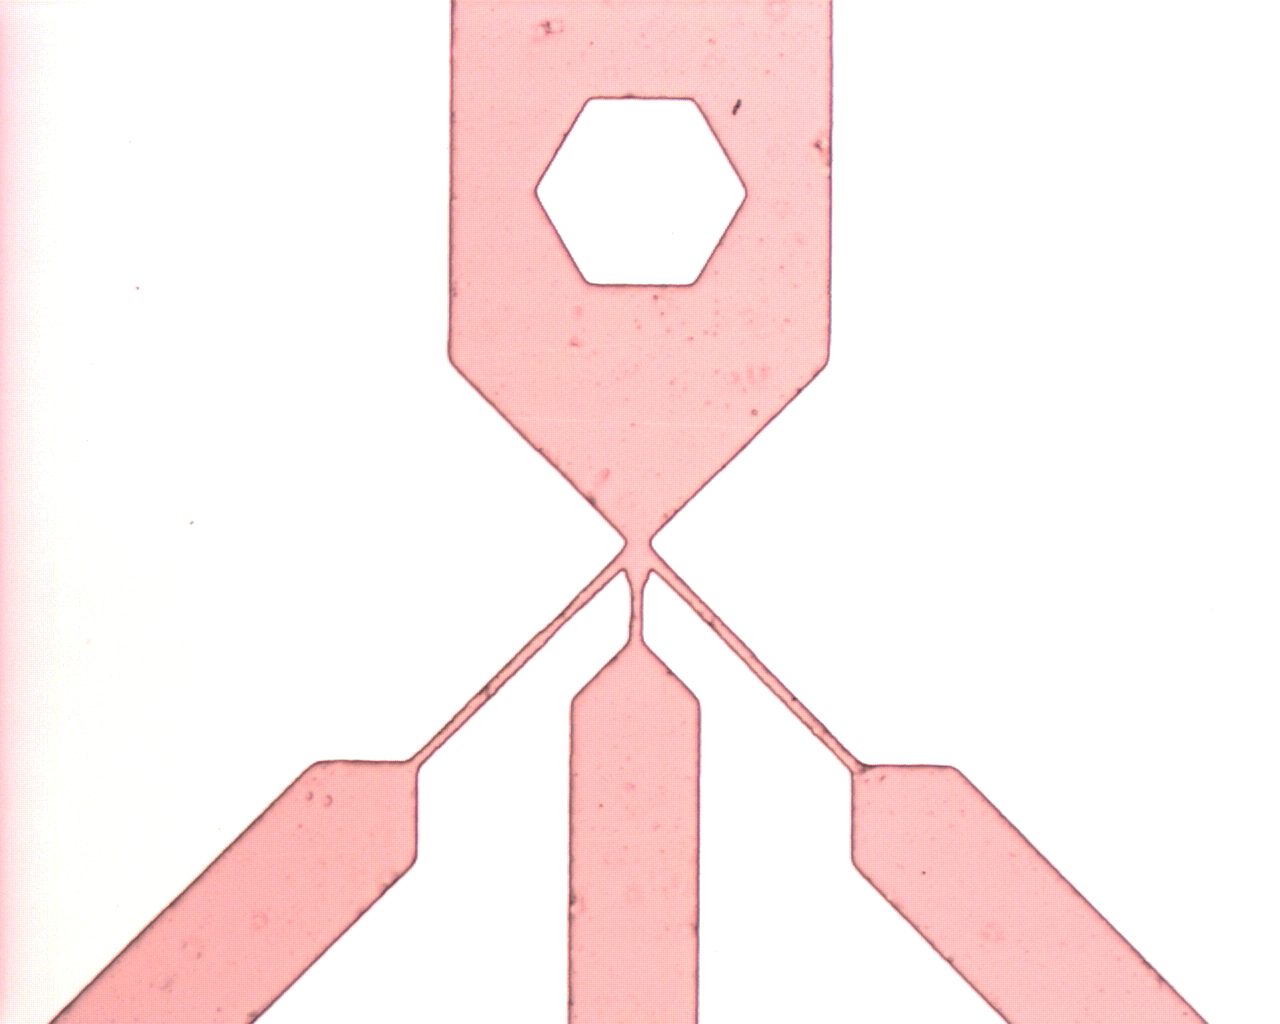
\includegraphics[width=0.8\textwidth]{images/su8_results.png}
    \caption{SU-8 photoresist as the master mold for PDMS micro-fluidic channels.}
    \label{fig:su8_results}
\end{figure}

\par The SU-8 master mold created through photolithography with the transparency mask, matched the transparency and the designed mold height closely. A representative SU-8 mold is depicted in figure \ref{fig:su8_results}. The dimensions of the SU-8 mold was verified using the Ambios Xp-1 profilometer. The SU-8 surface profile measured by the profilometer are presented in figure \ref{fig:profilometer_300um_channel} and \ref{fig:profilometer_10um_channel_100um_sideways}. 


\begin{figure}[H]
    \centering
    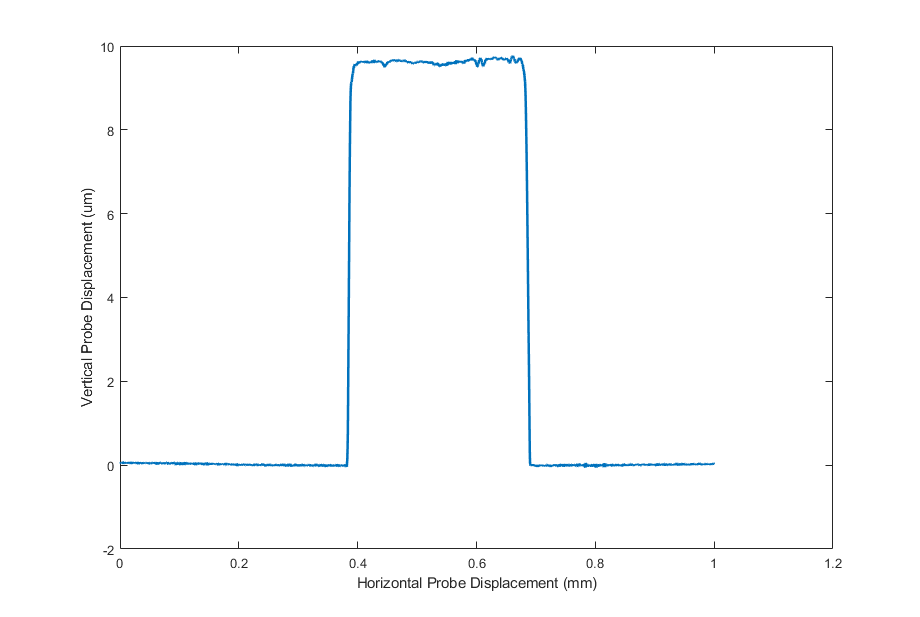
\includegraphics[width=\textwidth]{images/300umWideChannel.png}
    \caption[Surface profile of a 300 micron wide channel on the SU-8 master mold.]{Surface profile of a 300 micron wide channel on the SU-8 master mold. The profile was captured with the Ambios XP-1 profilometer. The profilometer recorded a channel height of 9.6 microns.}
    \label{fig:profilometer_300um_channel}
\end{figure}

\begin{figure}[h]
    \centering
    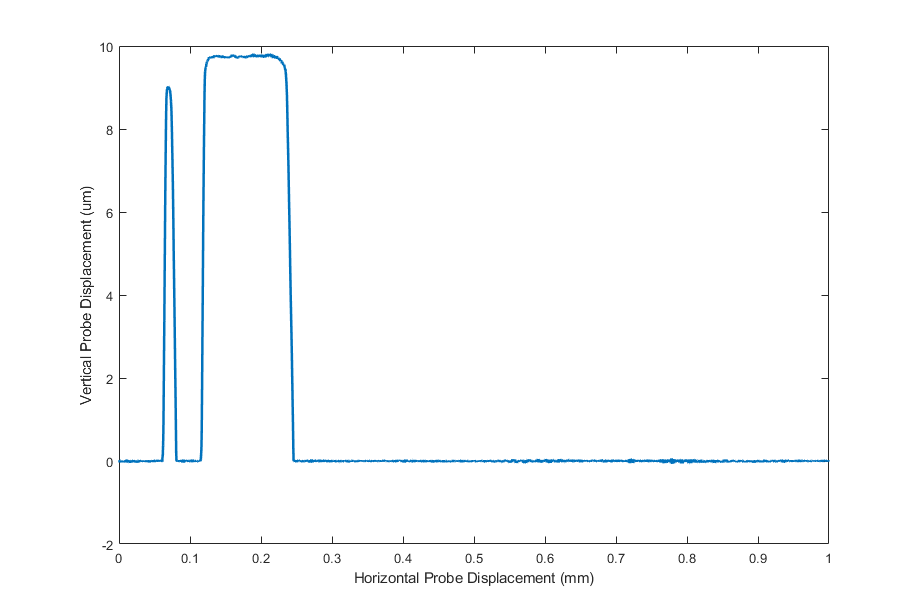
\includegraphics[width=\textwidth]{images/10umWideAndSidewaysThrough100umWide.png}
    \caption[Surface profile of a 10 micron and 100 micron wide channel on the SU-8 master mold.]{Surface profile of a 10 micron and 100 micron wide channel on the SU-8 master mold. The profile was captured with the Ambios XP-1 profilometer. The data depicts the 100 micron channel as about 140 microns wide since it crossed the channel at 45$^\circ$. The profilometer recorded a channel height of 9 and 9.6 microns for the 10 micron and 100 micron channels respectively.}
    \label{fig:profilometer_10um_channel_100um_sideways}
\end{figure}


\begin{figure}[H]
    \centering
    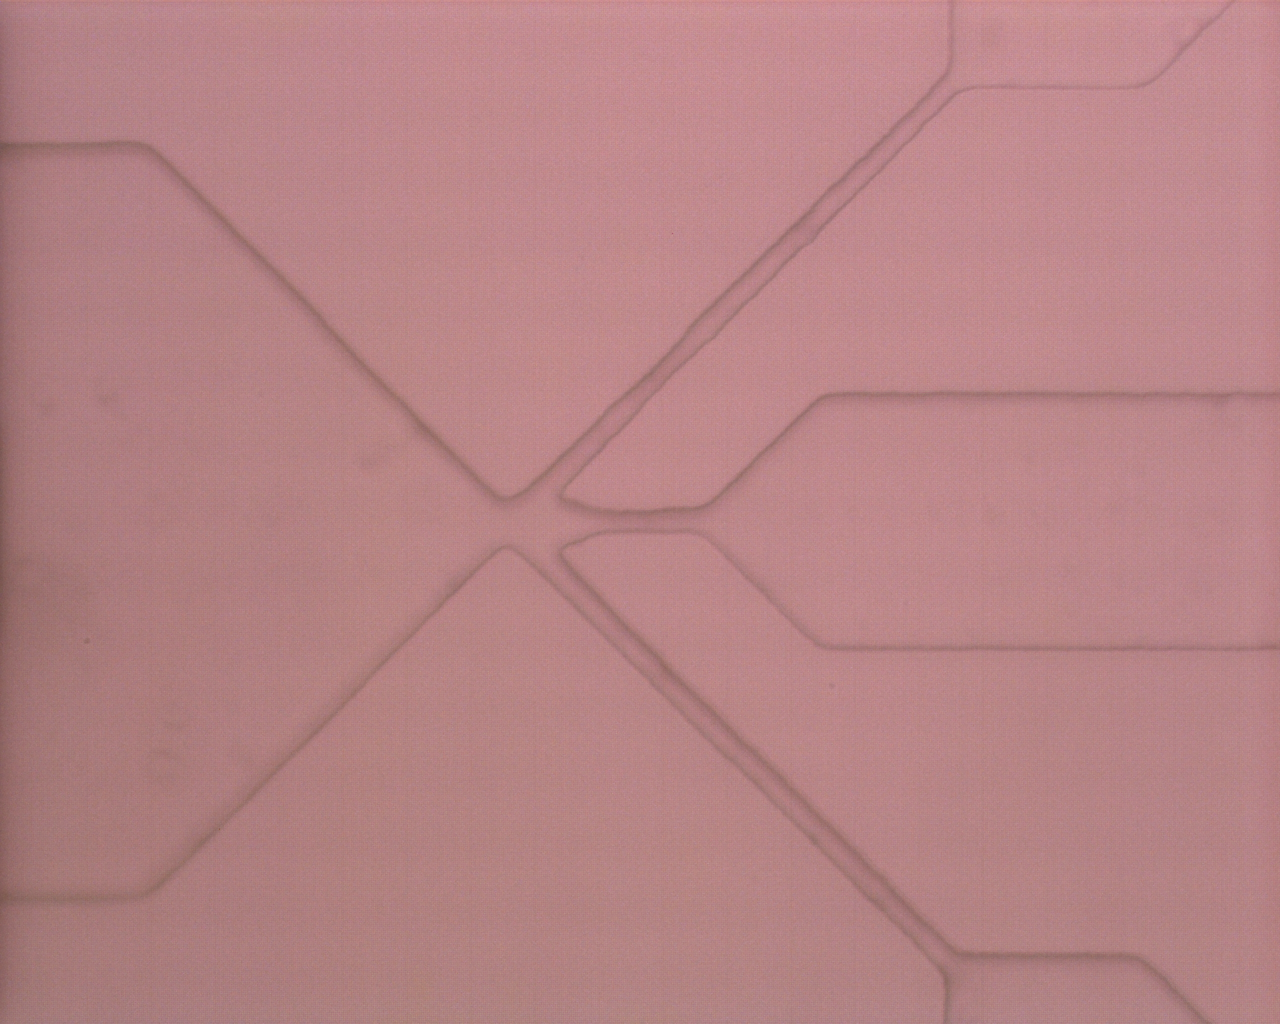
\includegraphics[width=0.9\textwidth]{images/PDMS_channels.png}
    \caption{PDMS cast from the master mold. Once bonded to a glass substrate, the cast will form the micro-fluidic channels of the device.}
    \label{fig:pdms_results}
\end{figure}

\FloatBarrier


\subsection{Electrode Fabrication}

\par Prior to this thesis, the micro-electrode fabrication process at Cal Poly was undeveloped and was developed through the course of this thesis. As a result, the fabrication process turned into an iterative approach of tuning process parameters and was met with many failures.

\begin{figure}[h]
    \centering
    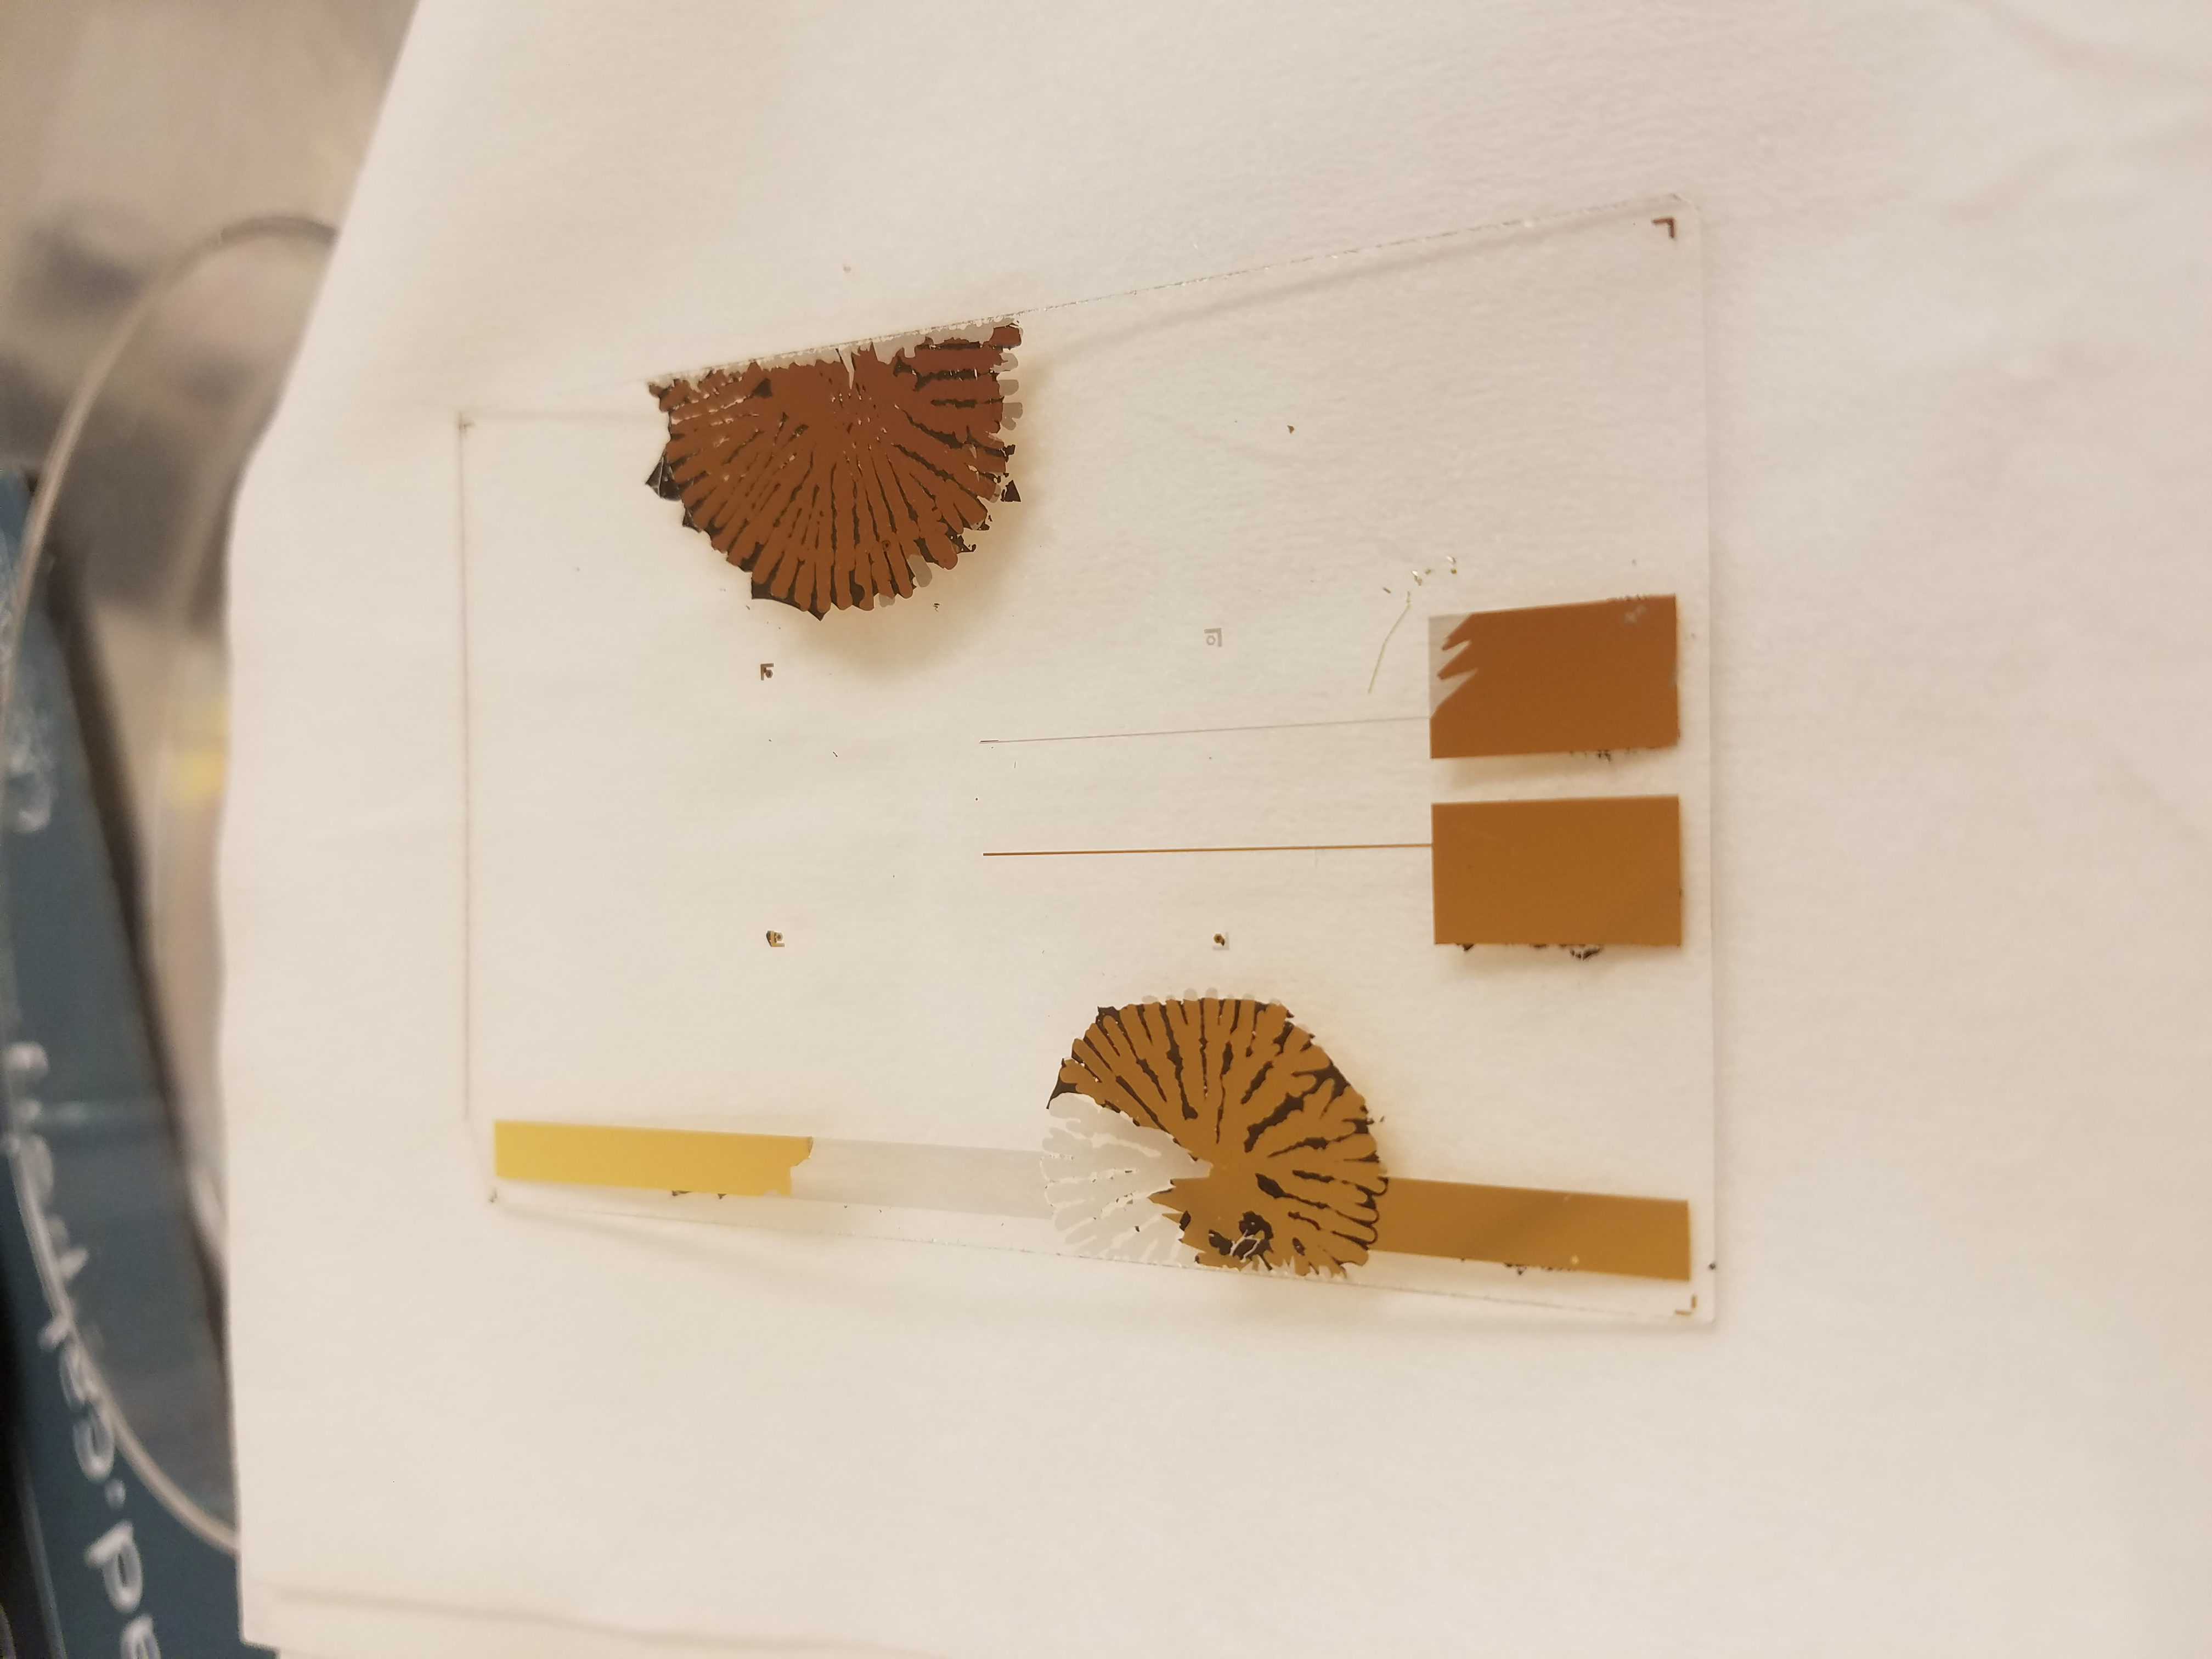
\includegraphics[width=\textwidth]{images/adhesion_issues.jpg}
    \caption{Electrode fabrication failure demonstrating two modes of failure: the Ma-N1420 photoresist failed to properly adhere to the glass surface manifesting as two anomalous flower patterns, and poor adhesion of the deposited gold to the first chrome layer as evident by gold-stripped leads.}
    \label{fig:failed_electrode_macro}
\end{figure}

\par Once the photolithography process was tuned, processed electrodes were met with three main modes of failure: poor photoresist adhesion, poor gold adhesion, and thin cracks or scrapes. 

\begin{figure}[h]
    \centering
    \begin{subfigure}[t]{0.45\textwidth}
        \centering
        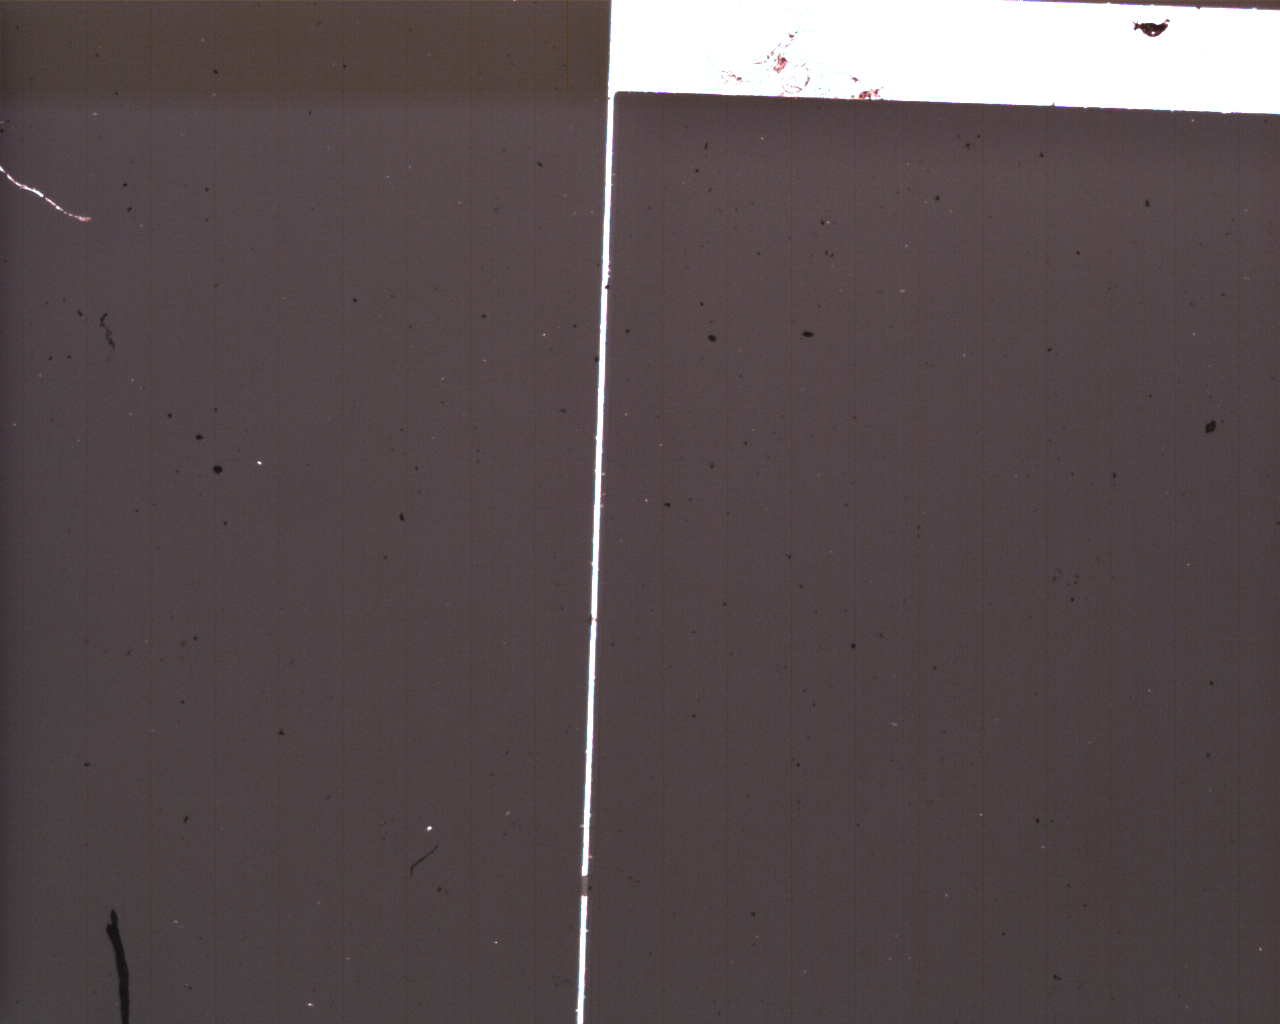
\includegraphics[width=\textwidth]{images/electrodeFailureChunkBreak.png}
        \caption{Break in electrode due to delamination of gold strip.}
    \end{subfigure}
    \hfill
    \begin{subfigure}[t]{0.45\textwidth}
        \centering
        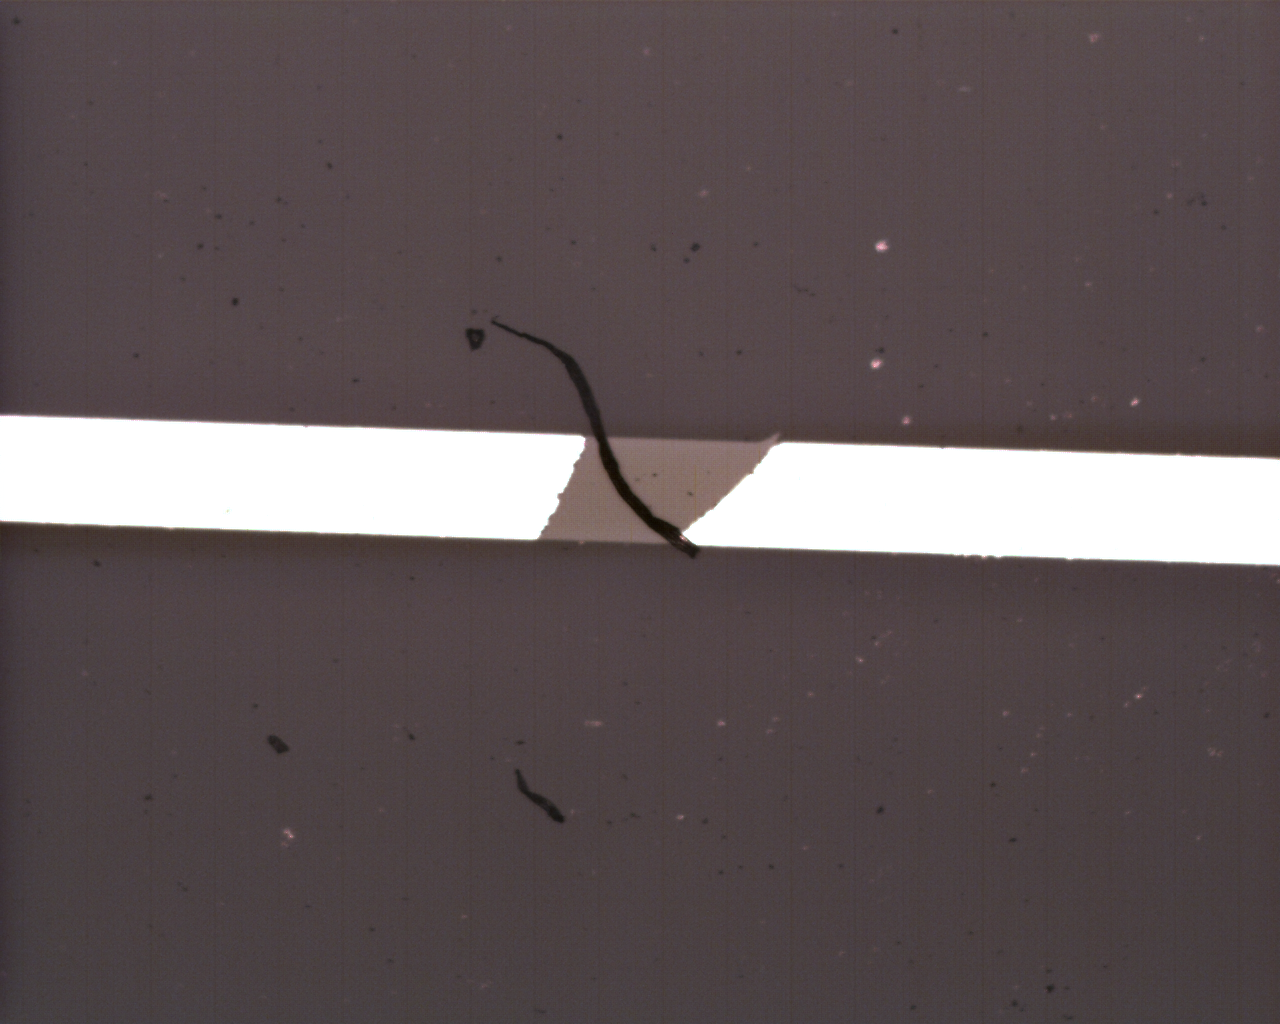
\includegraphics[width=\textwidth]{images/electrodeFailureChunkBreakZoomed.png}
        \caption{Visible chromium layer at site of electrode delamination highlights failure of gold adhesion to chromium layer.}
    \end{subfigure}
    \\
    \vspace{0.1 in}
    \begin{subfigure}[t]{0.45\textwidth}
        \centering
        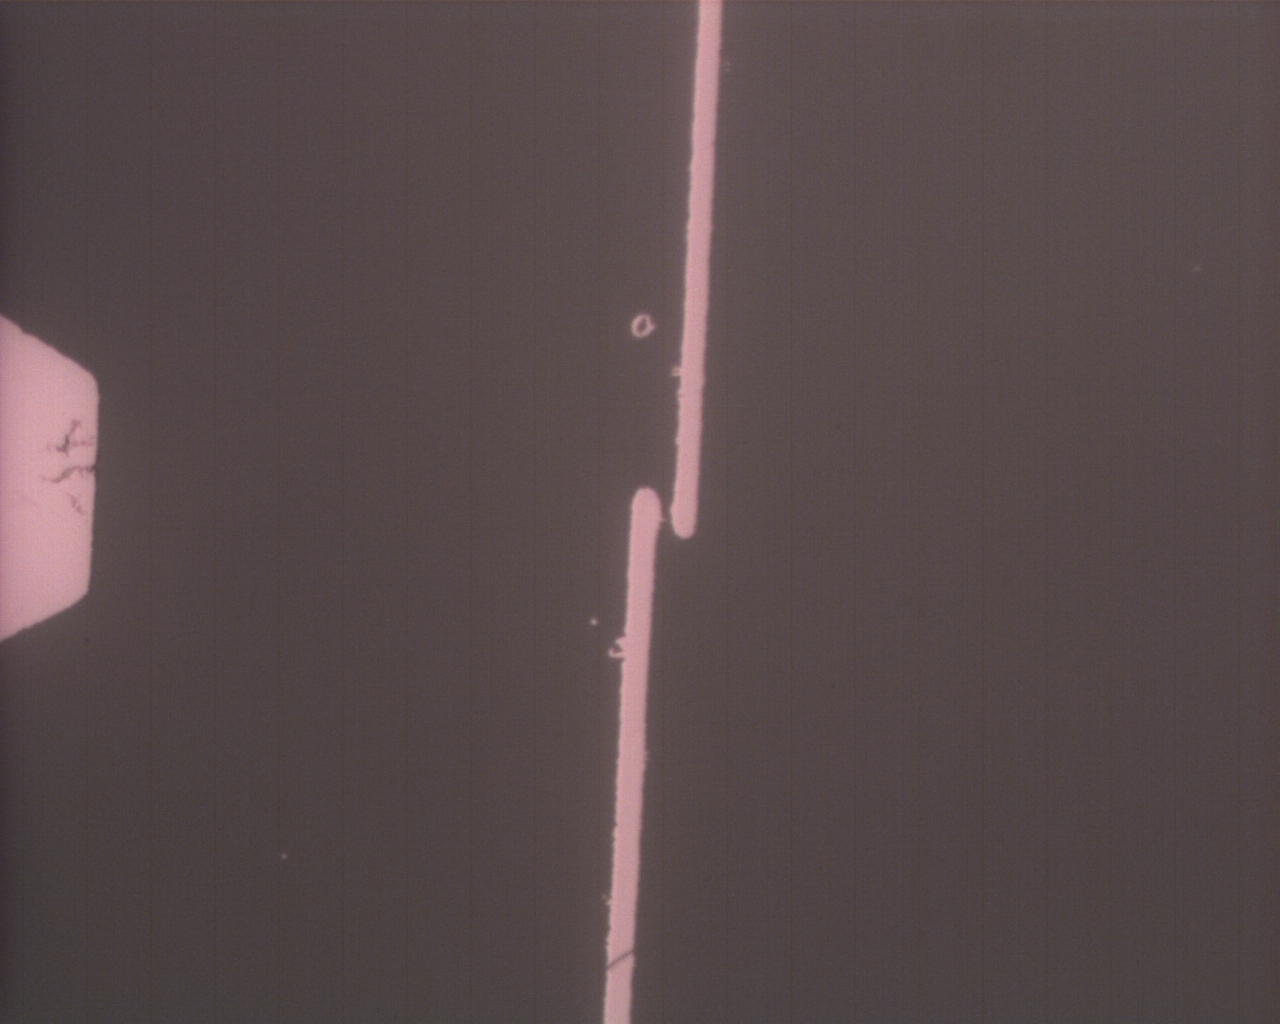
\includegraphics[width=\textwidth]{images/electrodeFailureThinBreak.png}
        \caption{Thin crack in electrode.}
    \end{subfigure}
    \hfill
    \begin{subfigure}[t]{0.45\textwidth}
        \centering
        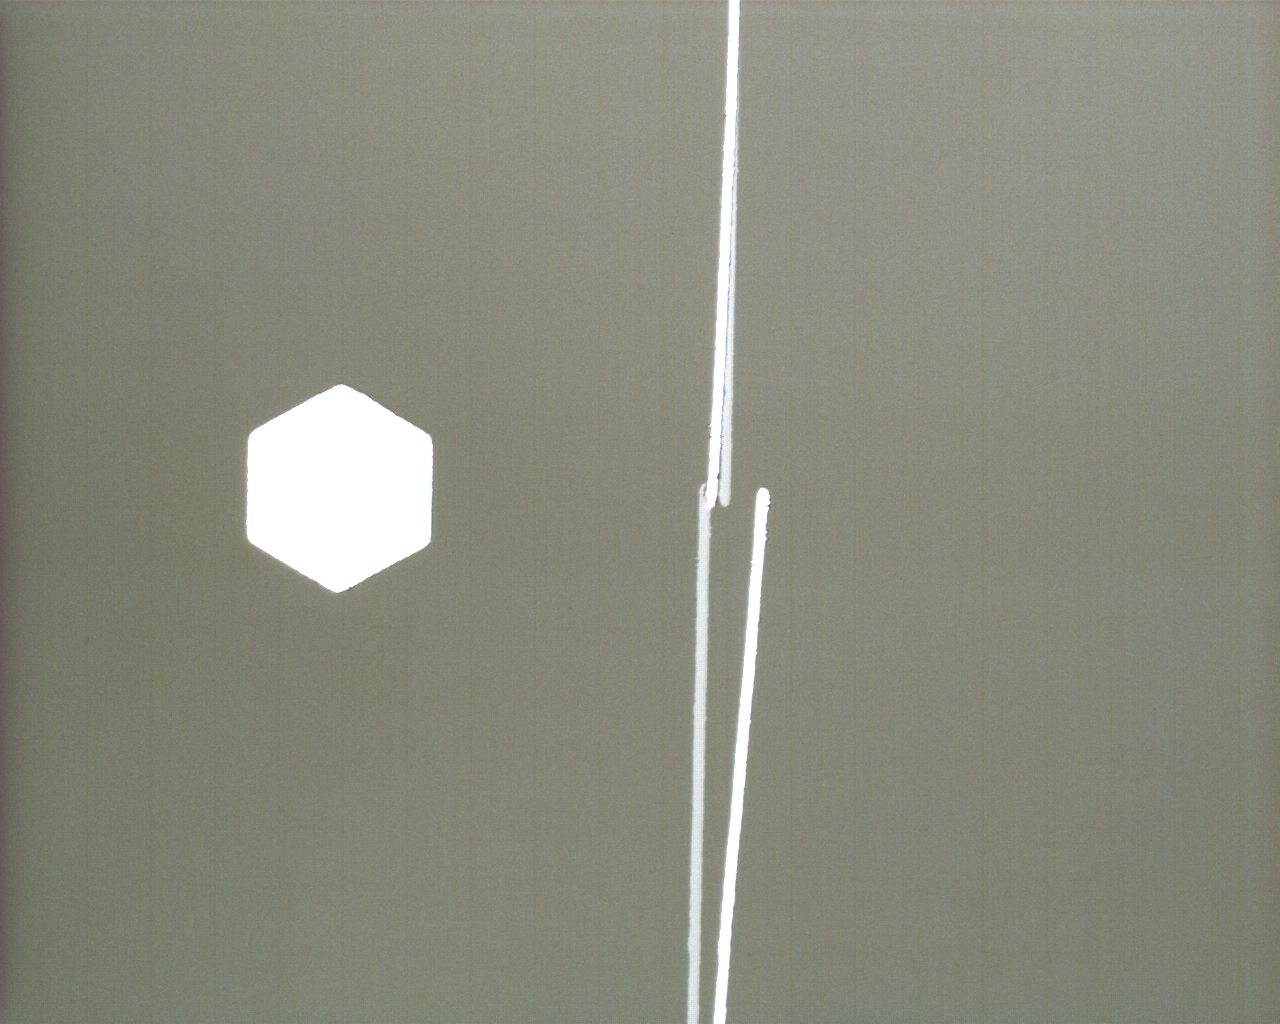
\includegraphics[width=\textwidth]{images/electrodeFailureSlide.png}
        \caption{Gold electrode strips sliding off chrome adhesion layer}
    \end{subfigure}
    \caption{Images of common electrode fabrication failures.}
    \label{fig:failed_elecftrodes_micro}
\end{figure}

\begin{figure}[h]
    \begin{subfigure}[b]{\textwidth}
        \centering
        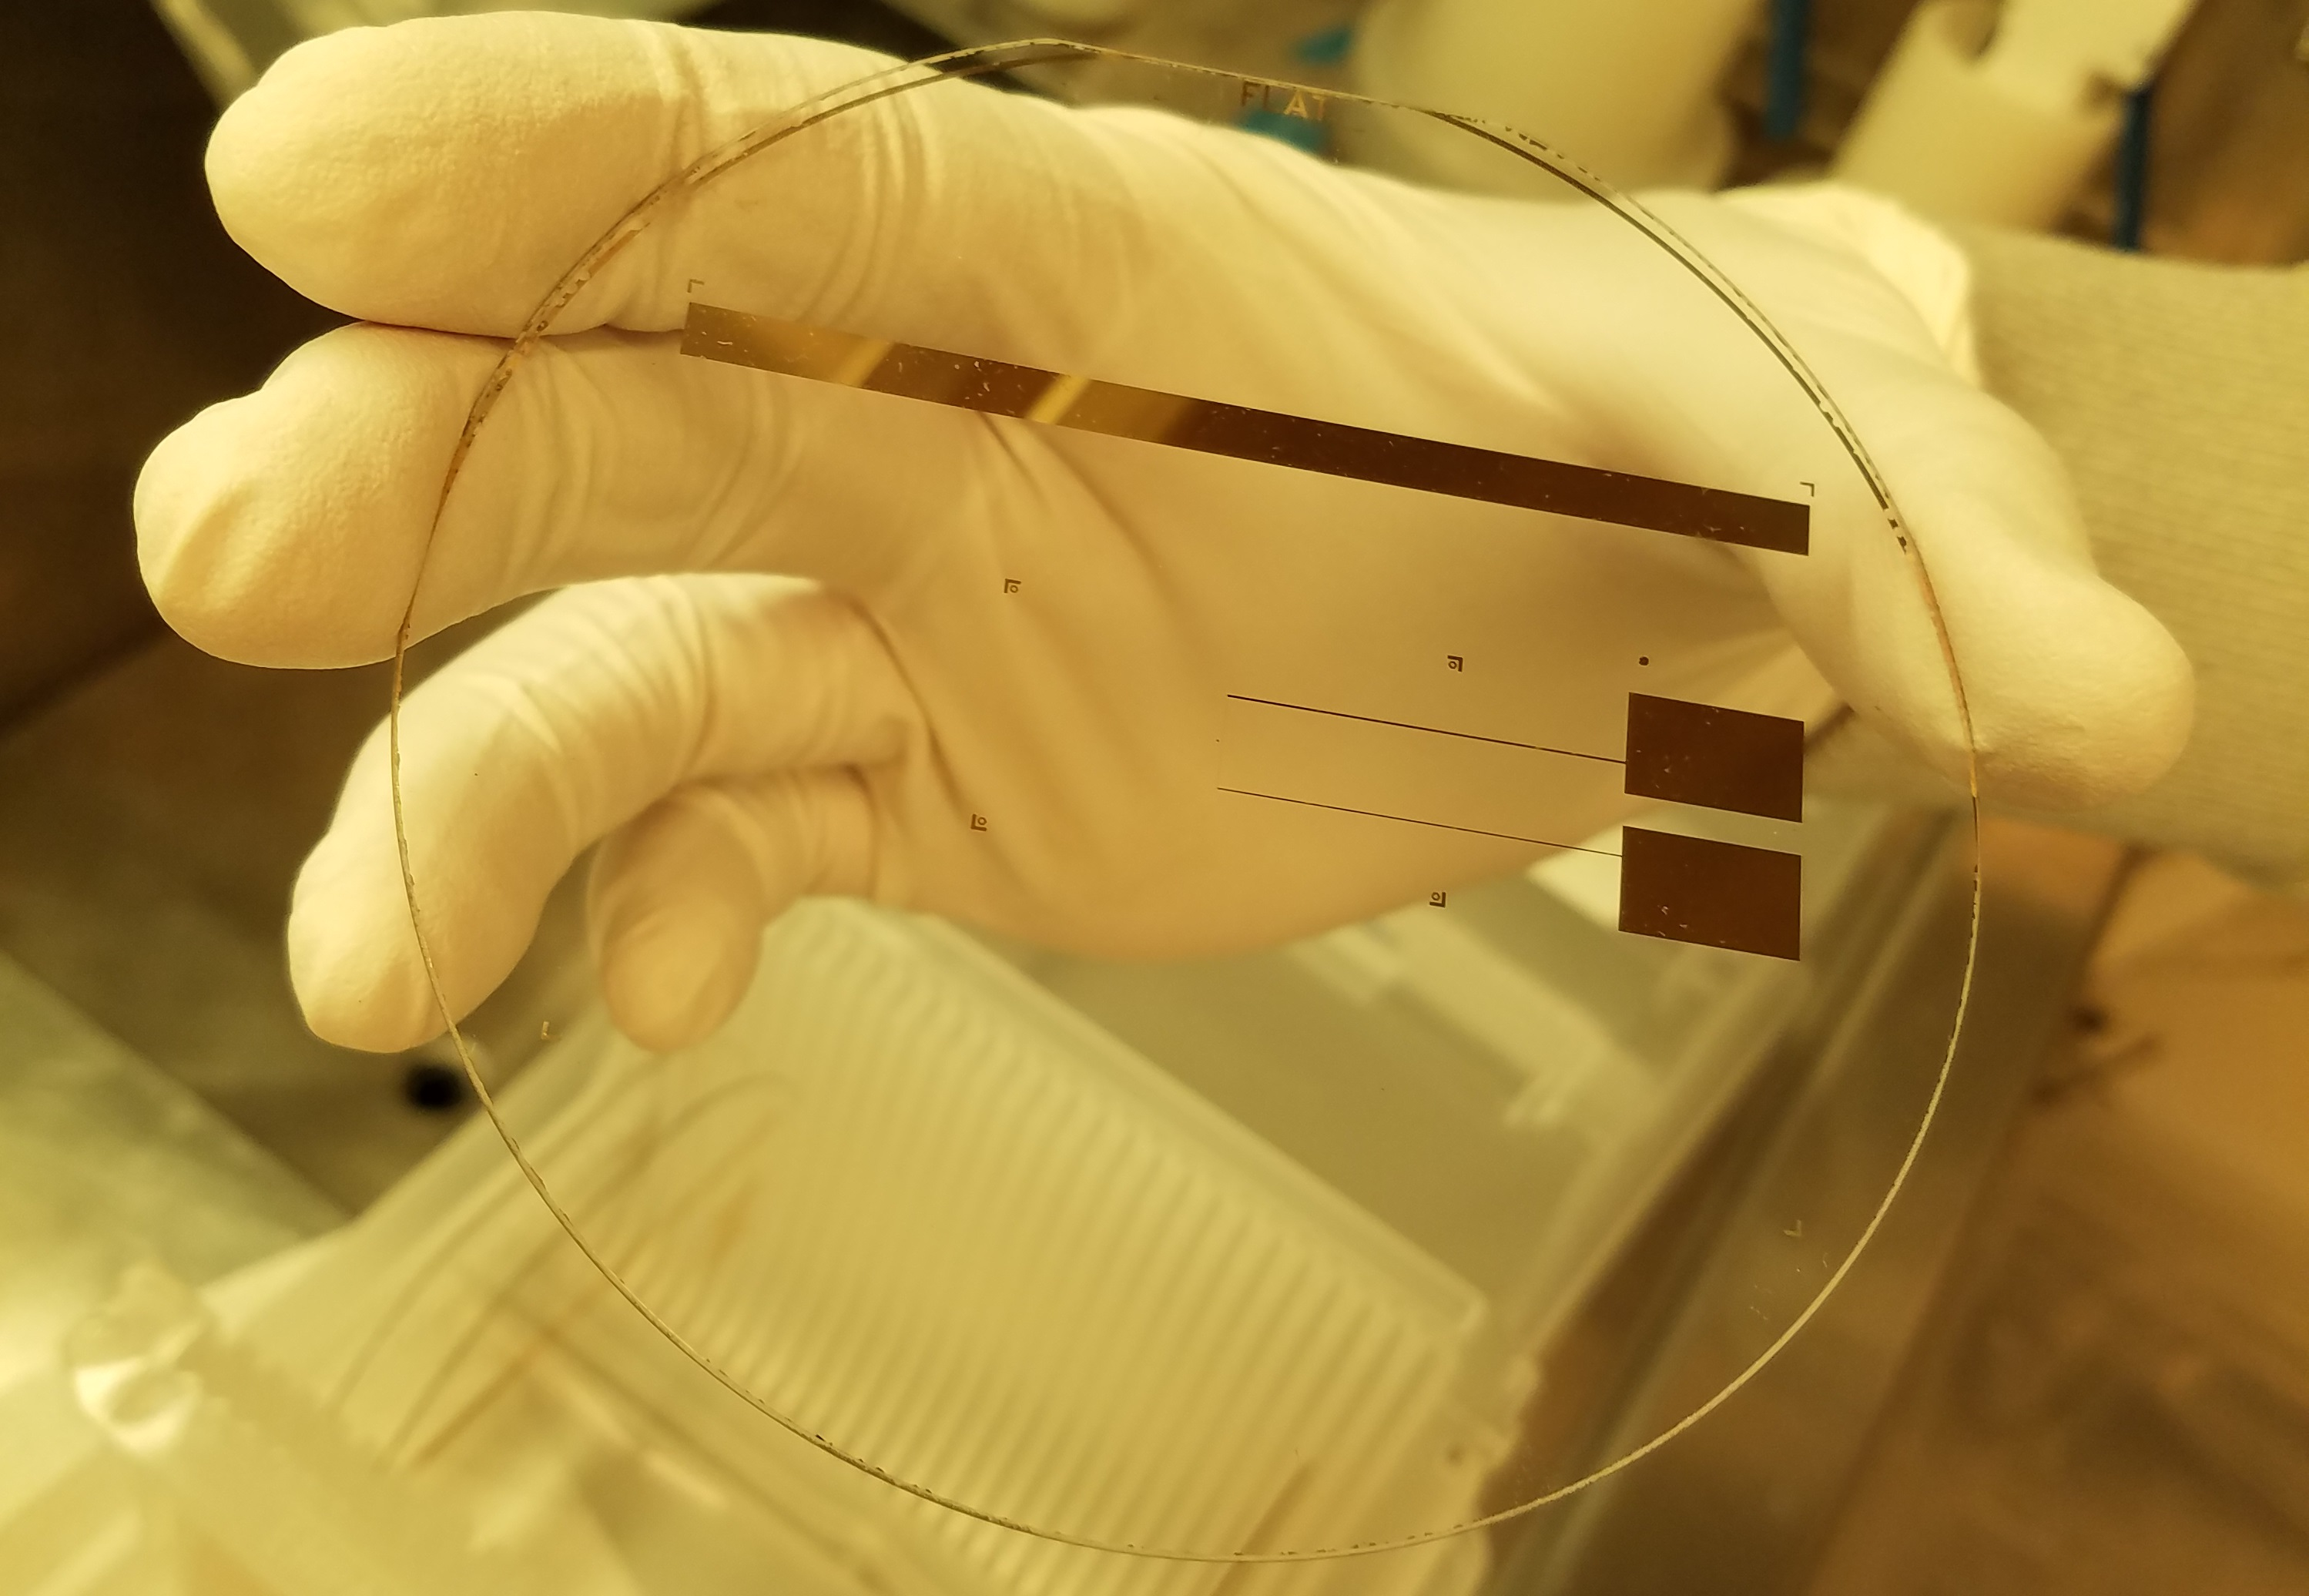
\includegraphics[width=\textwidth]{images/electrodes_real.jpg}
        \caption{Successful fabrication of device electrodes}
    \end{subfigure}
    \\
    \vspace{0.1 in}
    \centering
    \begin{subfigure}[b]{0.45\textwidth}
        \centering
        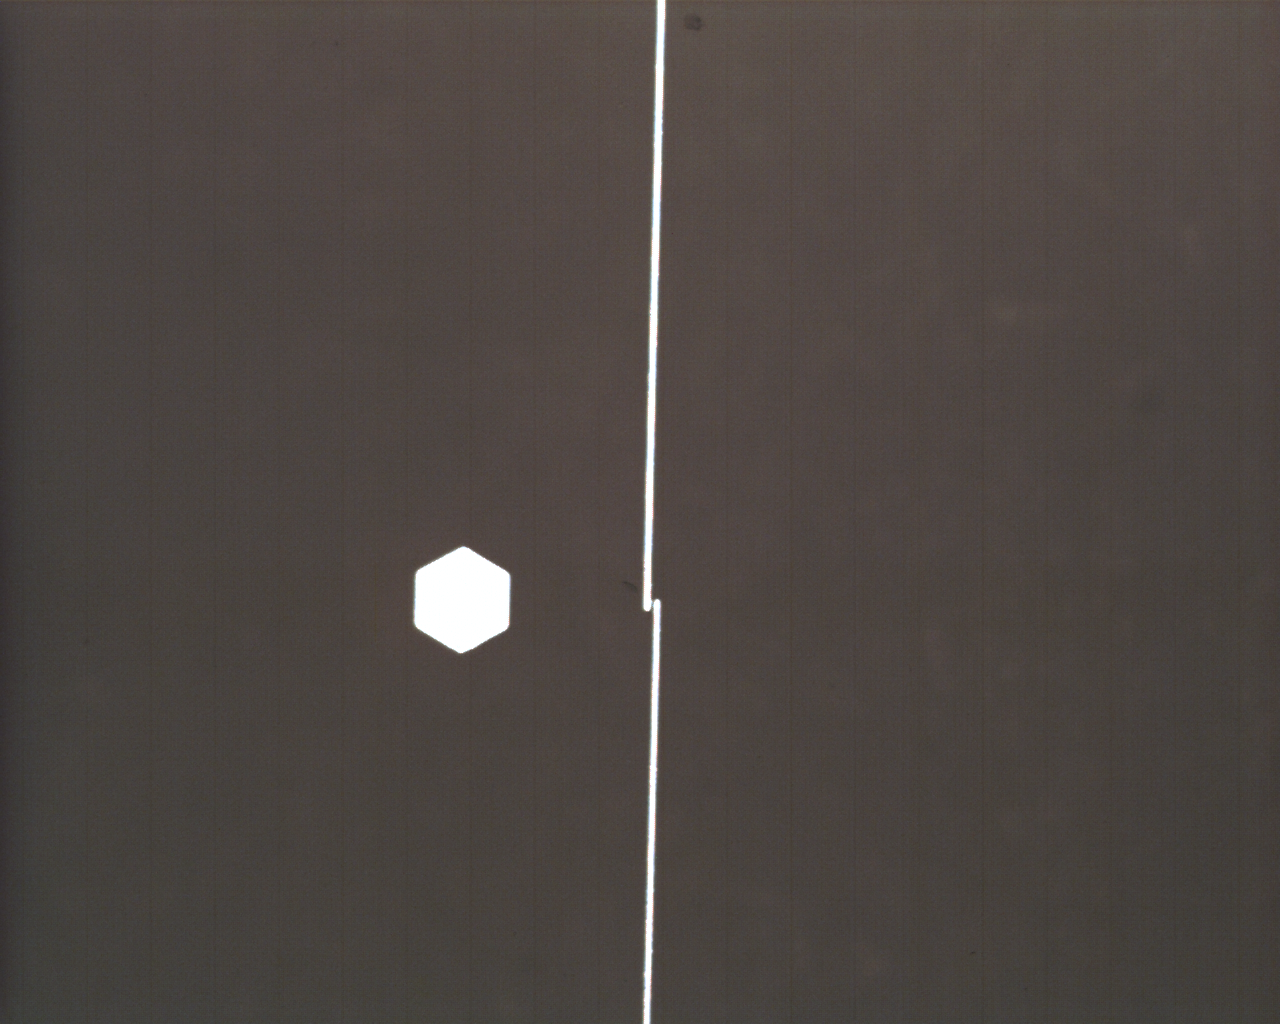
\includegraphics[width=\textwidth]{images/goodElectrode.png}
        \caption{Impedance magnitude and phase}
    \end{subfigure}
    \hfill
    \begin{subfigure}[b]{0.45\textwidth}
        \centering
        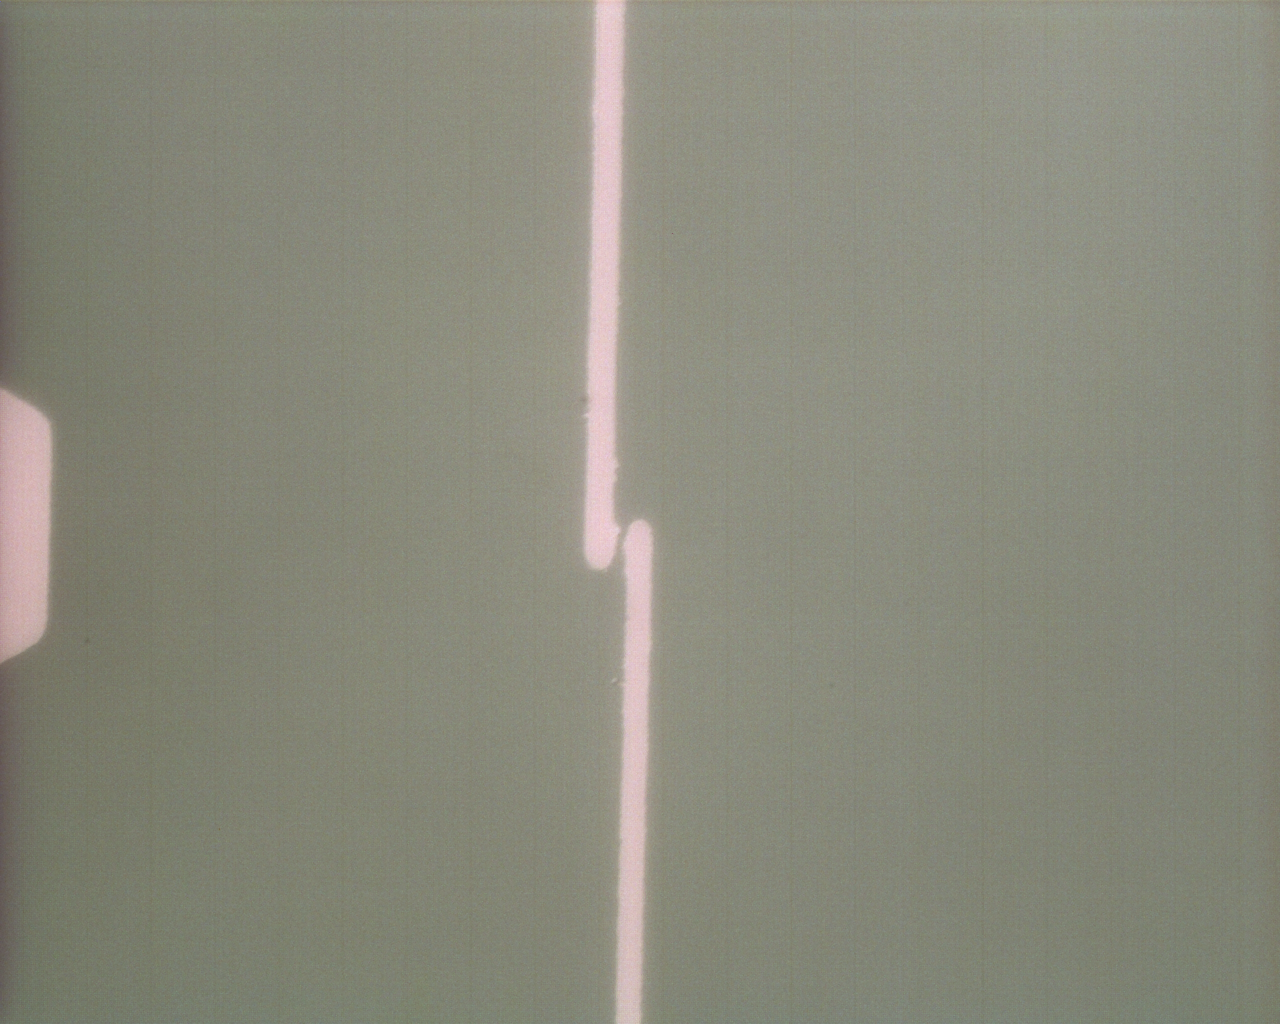
\includegraphics[width=\textwidth]{images/goodElectrodeCloseUp.png}
        \caption{Real and imaginary impedance}
    \end{subfigure}
    \caption{Integral electrodes with no breaks in sputtered gold layer. The successful results were realized by minimizing the exposure of the chromium adhesion layer to air and reducing the formation chromium oxide.}
\end{figure}


\FloatBarrier

\subsection{Device Bonding}


\begin{figure}[h]
    \centering
    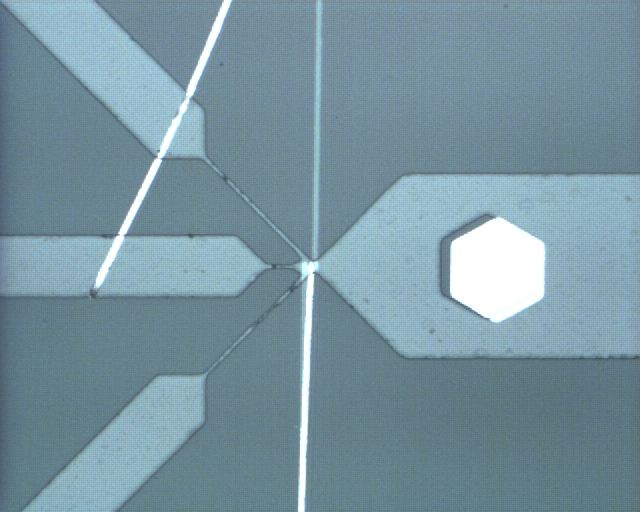
\includegraphics[width=\textwidth]{images/bad_device.png}
    \caption{Electrode adhesion failure during plasma bonding process of device 1. The sputtered gold layer delaminated from the chromium adhesion layer during PDMS to electrode alignment.}
    \label{fig:bad_device}
\end{figure}


\begin{figure}[h]
    \centering
    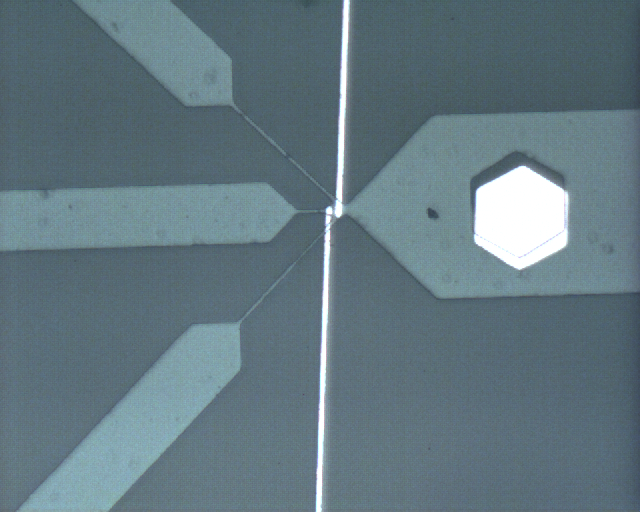
\includegraphics[width=\textwidth]{images/good_device.png}
    \caption{Successfully bonded impedance spectroscopy device. PDMS and electrodes were aligned by hand. There is a slight rotational misalignment, but should be functionally negligible.}
    \label{fig:good_device}
\end{figure}

\FloatBarrier

\section{Impedance Spectroscopy System}

\begin{figure}[h]
    \centering
    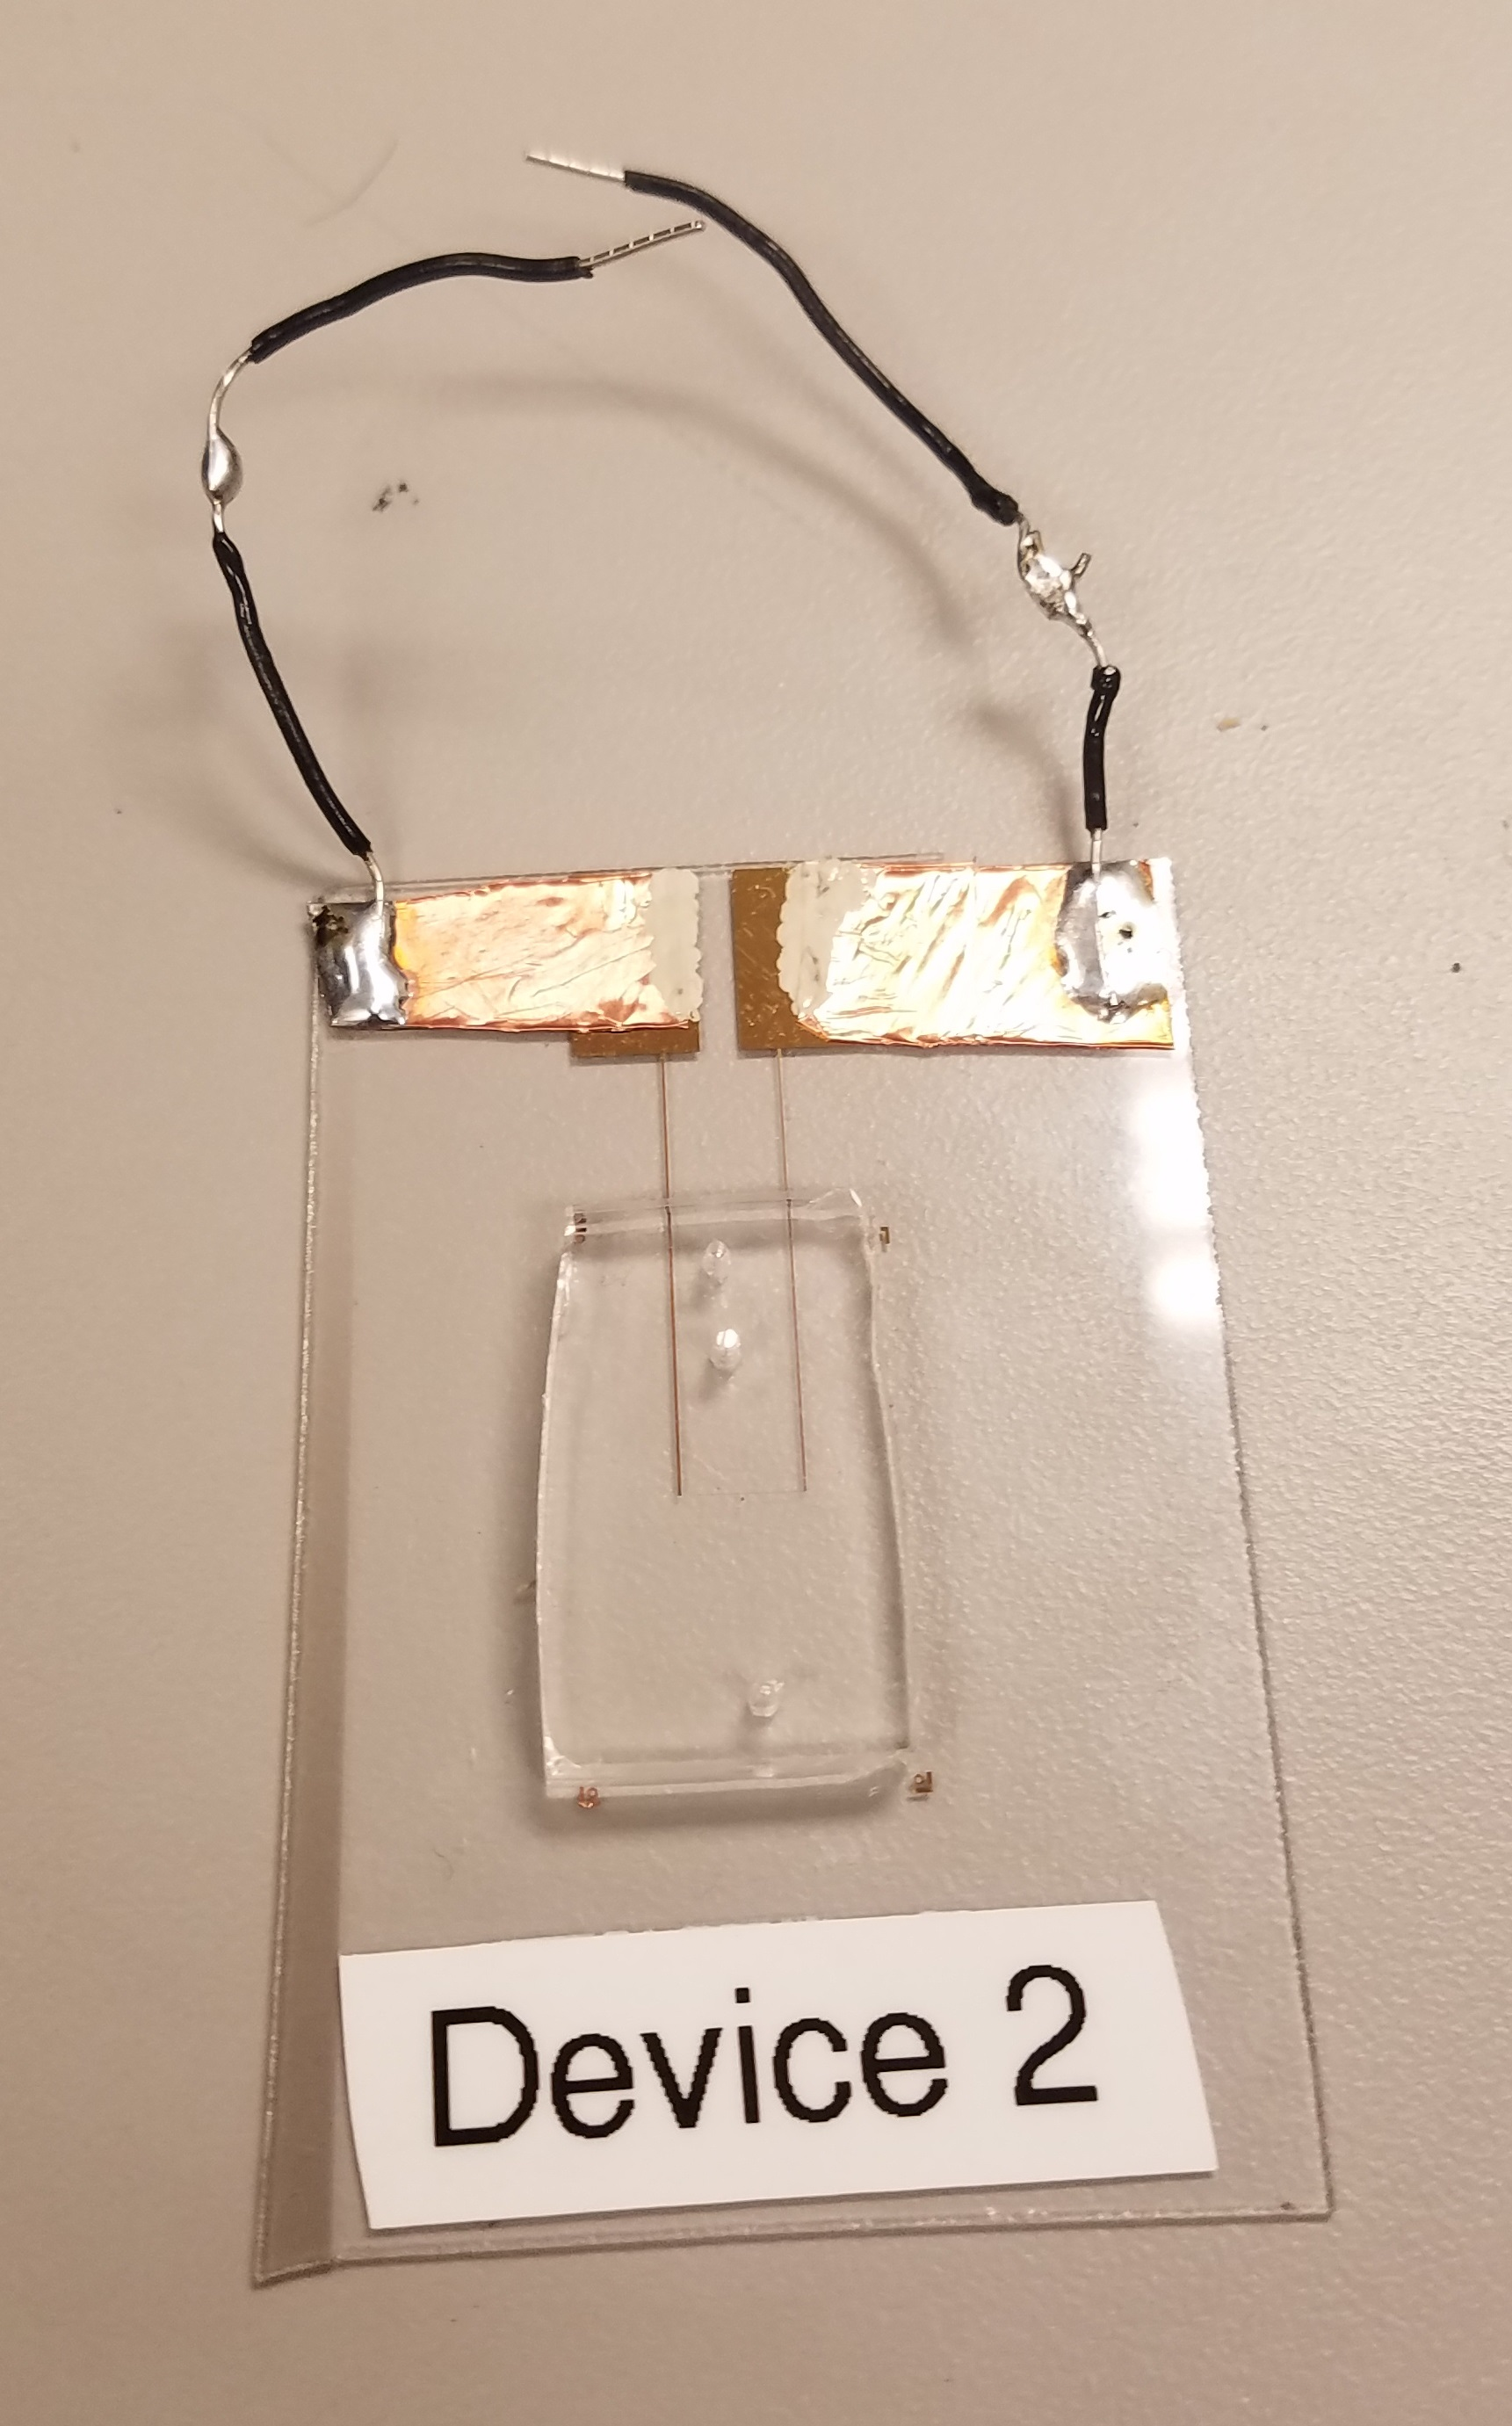
\includegraphics[width=0.5\textwidth]{images/device_22.jpg}
    \caption{Successfully assembled cell impedance spectroscopy device.}
    \label{fig:my_label}
\end{figure}

\begin{figure}[h]
    \centering
    \begin{subfigure}[b]{0.45\textwidth}
        \centering
        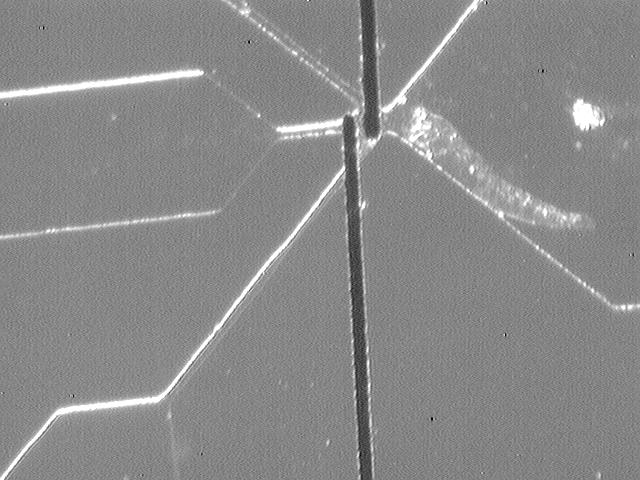
\includegraphics[width=\textwidth]{images/IS_empty.jpg}
        \caption{Sensor chamber saturated with phosphate buffered solution.}
    \end{subfigure}
    \hfill
    \begin{subfigure}[b]{0.45\textwidth}
        \centering
        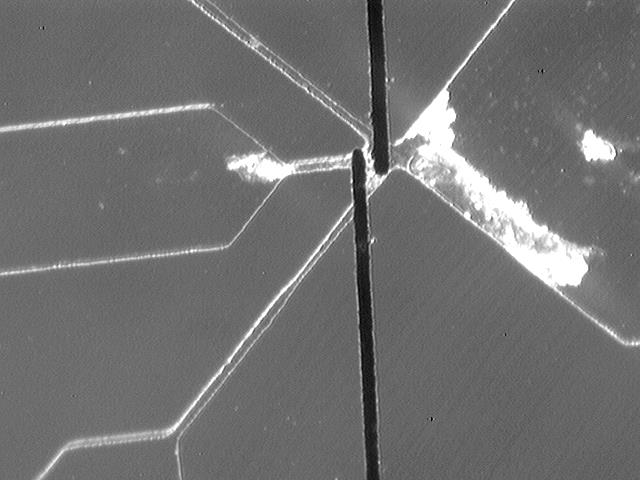
\includegraphics[width=\textwidth]{images/IS_particle_saturation.jpg}
        \caption{Sensor chamber saturated with7$\mu$m polystyrene beads.}
    \end{subfigure}
    \\
    \vspace{0.1 in}
    \begin{subfigure}[b]{0.45\textwidth}
        \centering
        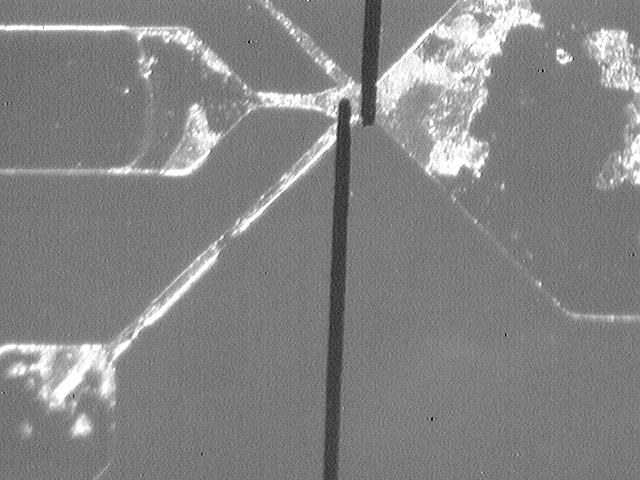
\includegraphics[width=\textwidth]{images/IS_jammed.jpg}
        \caption{Sensor region jammed with debris and beads.}
    \end{subfigure}
    \hfill
    \begin{subfigure}[b]{0.45\textwidth}
        \centering
        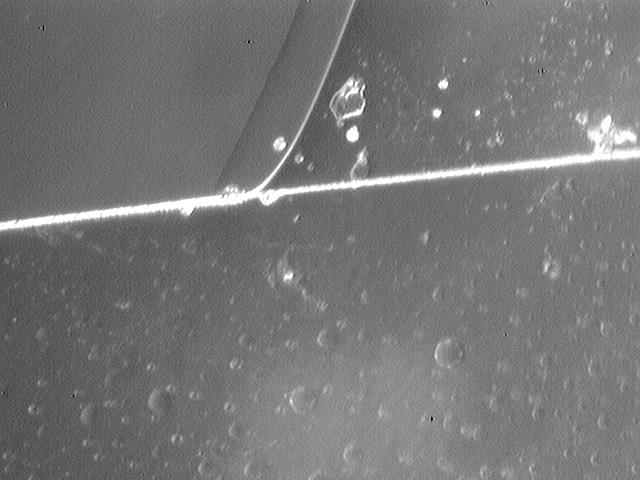
\includegraphics[width=\textwidth]{images/IS_device_delamination.jpg}
        \caption{Device delaminated after attempt to flush jammed sensor region.}
    \end{subfigure}
    \caption{Images of the sensor region of the impedance spectroscopy device. The device successfully measured fluid and 7 $\mu$m beads before the sensor region became jammed and the device ultimately delaminated. Images were taken with the LabSmith SVM340 inverted microscope.}
    \label{fig:IS_sensor_reigon_measurement}
\end{figure}

\begin{figure}[h]
    \centering
    \begin{subfigure}[b]{\textwidth}
        \centering
        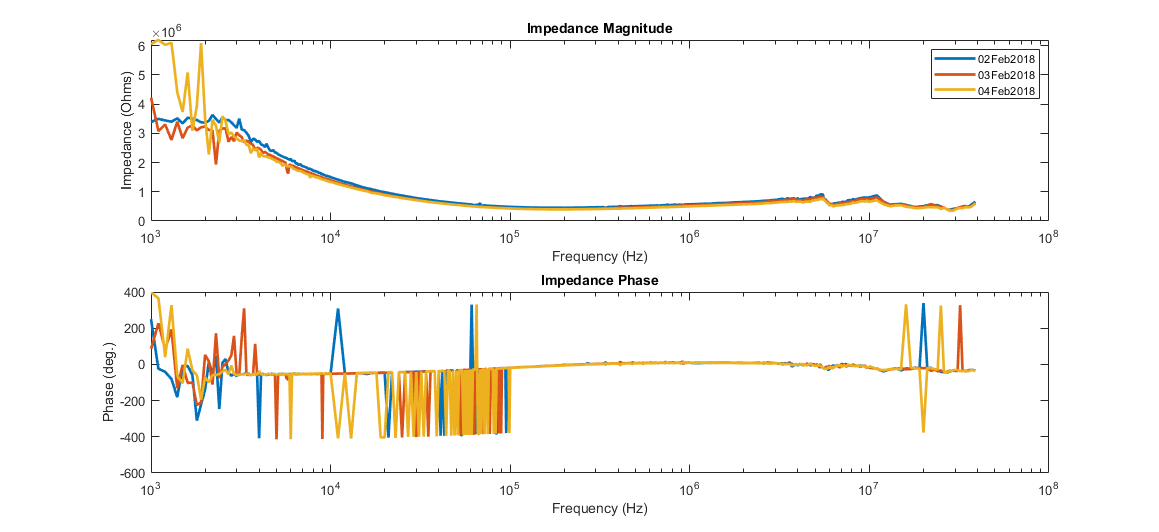
\includegraphics[width=\textwidth]{images/reproducibility_PBS_mag_phase.png}
        \caption{PBS impedance spectroscopy results in polar form.}
    \end{subfigure}
    \\
    \vspace{0.1 in}
    \begin{subfigure}[b]{\textwidth}
        \centering
        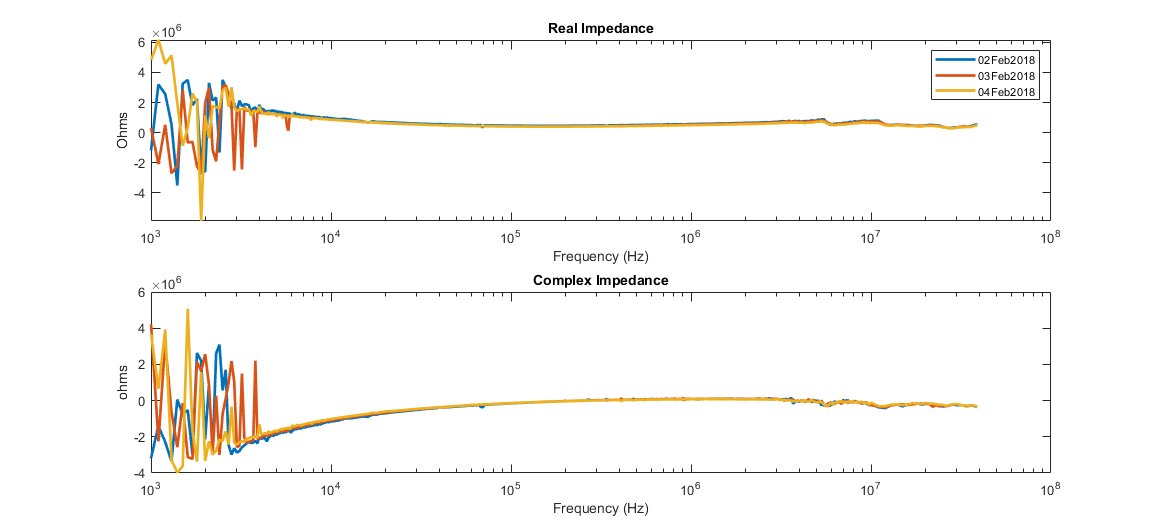
\includegraphics[width=\textwidth]{images/reproducibility_PBS_real_imag.png}
        \caption{PBS impedance spectroscopy results in rectangular form.}
    \end{subfigure}
    \caption{Reproducibility of the demonstrated with repeated measurement of phosphate buffered solution over a span of three days.}
    \label{fig:IS_data_reproducibility}
\end{figure}

\begin{figure}[h]
    \centering
    \begin{subfigure}[b]{\textwidth}
        \centering
        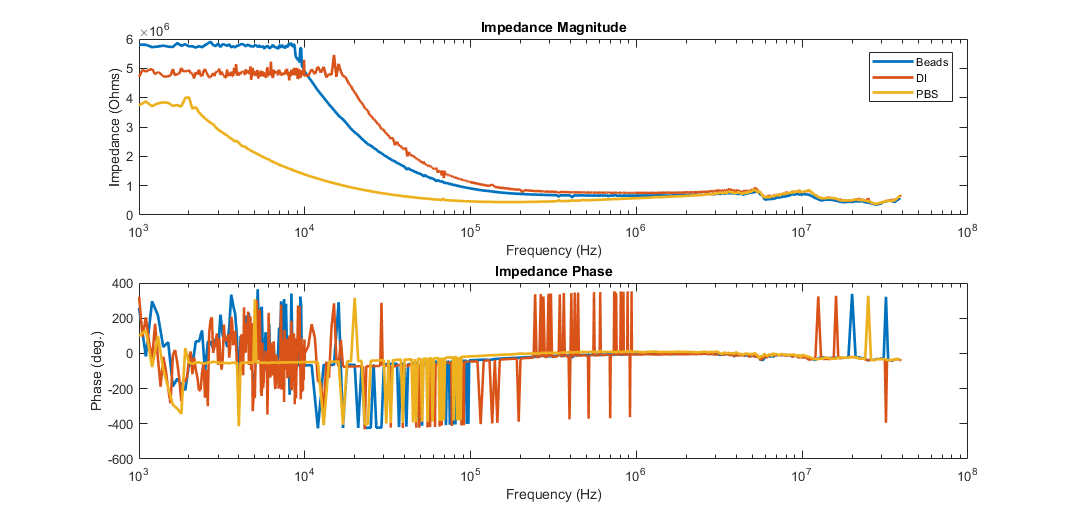
\includegraphics[width=\textwidth]{images/raw_IS_data_mag_phase.png}
        \caption{Impedance spectroscopy results in polar form.}
    \end{subfigure}
    \\
    \vspace{0.1 in}
    \begin{subfigure}[b]{\textwidth}
        \centering
        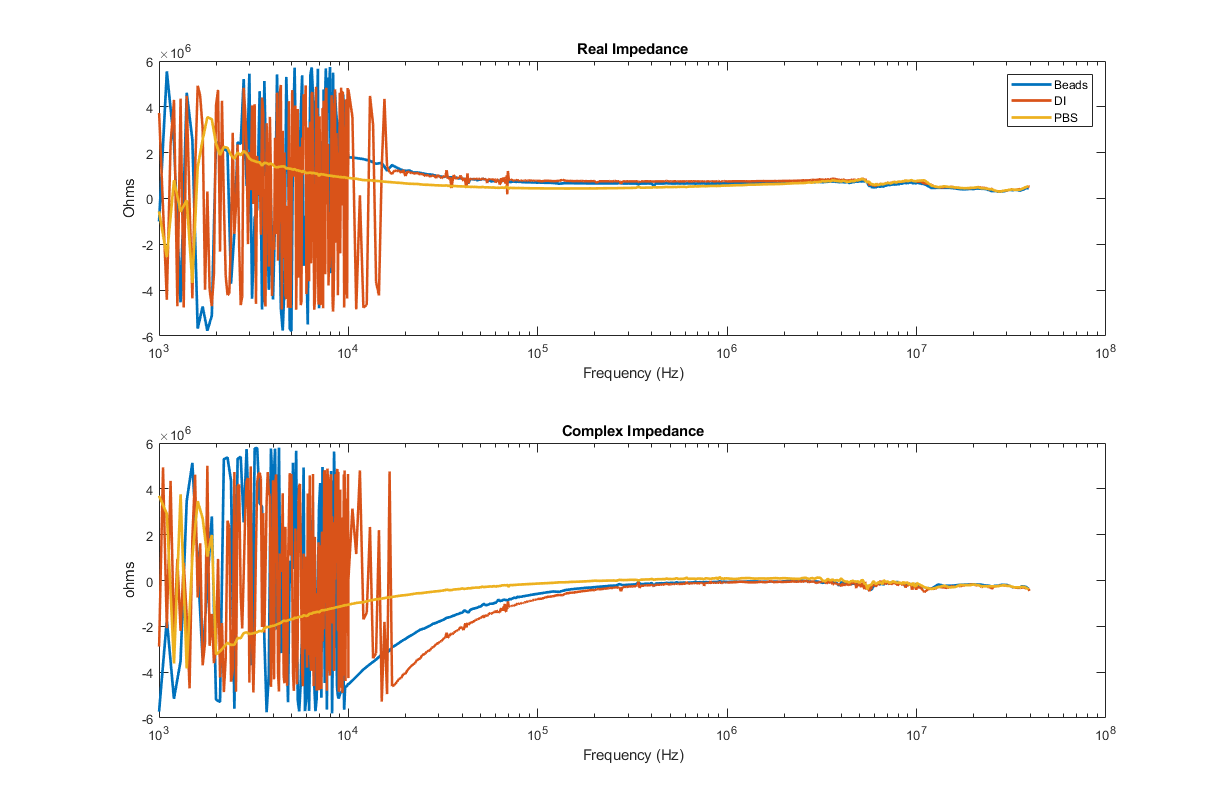
\includegraphics[width=\textwidth]{images/raw_IS_data_real_imag.png}
        \caption{Impedance spectroscopy results in rectangular form.}
    \end{subfigure}
    \\
%    \vspace{0.1 in}
%    \begin{subfigure}[b]{\textwidth}
%        \centering
%        \includegraphics[width=\textwidth]{images/raw_IS_%data_nyquist.png}
%        \caption{Jammed}
%    \end{subfigure}
    \caption[PBS, DI, microbead IS Raw data comparison.]{Comparison of impedance spectroscopy results using raw measurements of phosphate buffered solution, de-ionized water, and the chamber saturated with 7 $\mu$m polystyrene beads.}
    \label{fig:IS_data_beads_pbs_DI_comp}
\end{figure}

\begin{figure}[h]
    \centering
    \begin{subfigure}[b]{\textwidth}
        \centering
        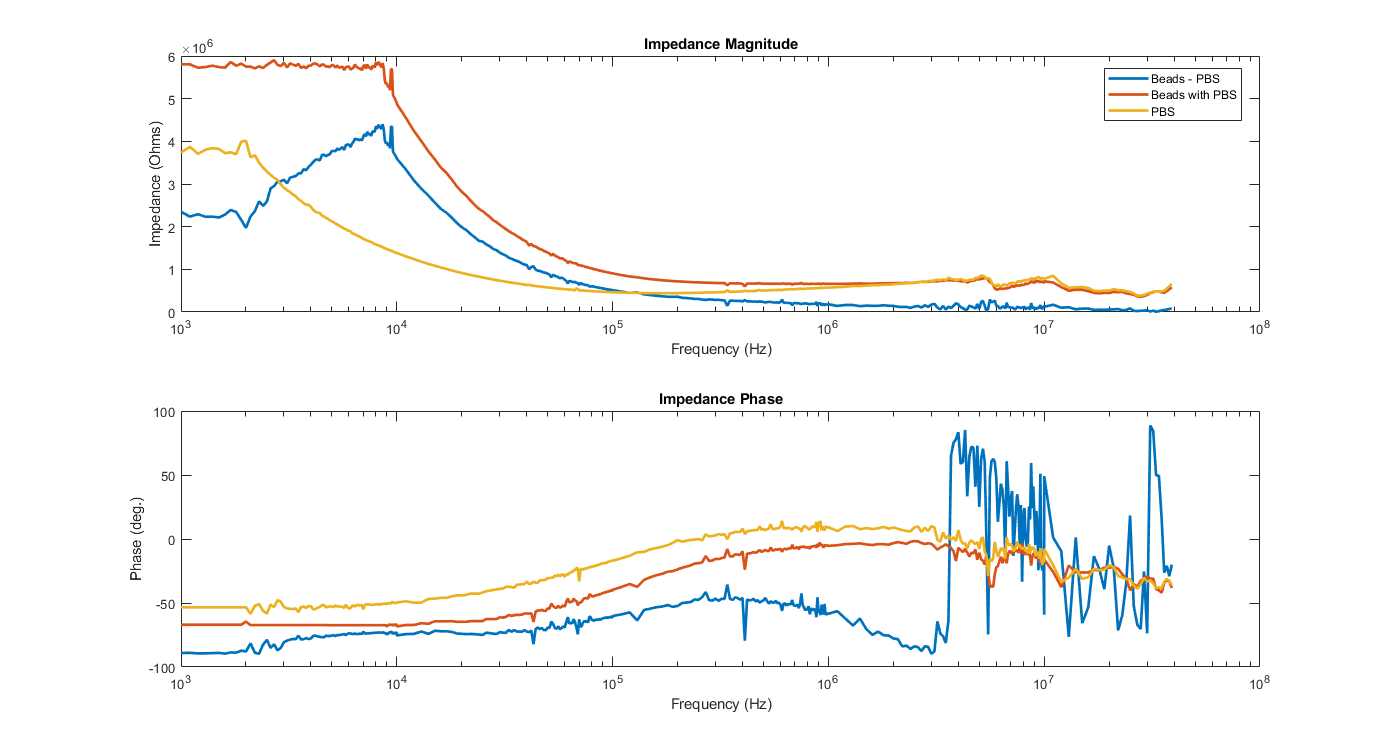
\includegraphics[width=\textwidth]{images/IS_data_clean_mag_phase.png}
        \caption{IS results in polar form.}
    \end{subfigure}
    \\
    \vspace{0.1 in}
    \begin{subfigure}[b]{\textwidth}
        \centering
        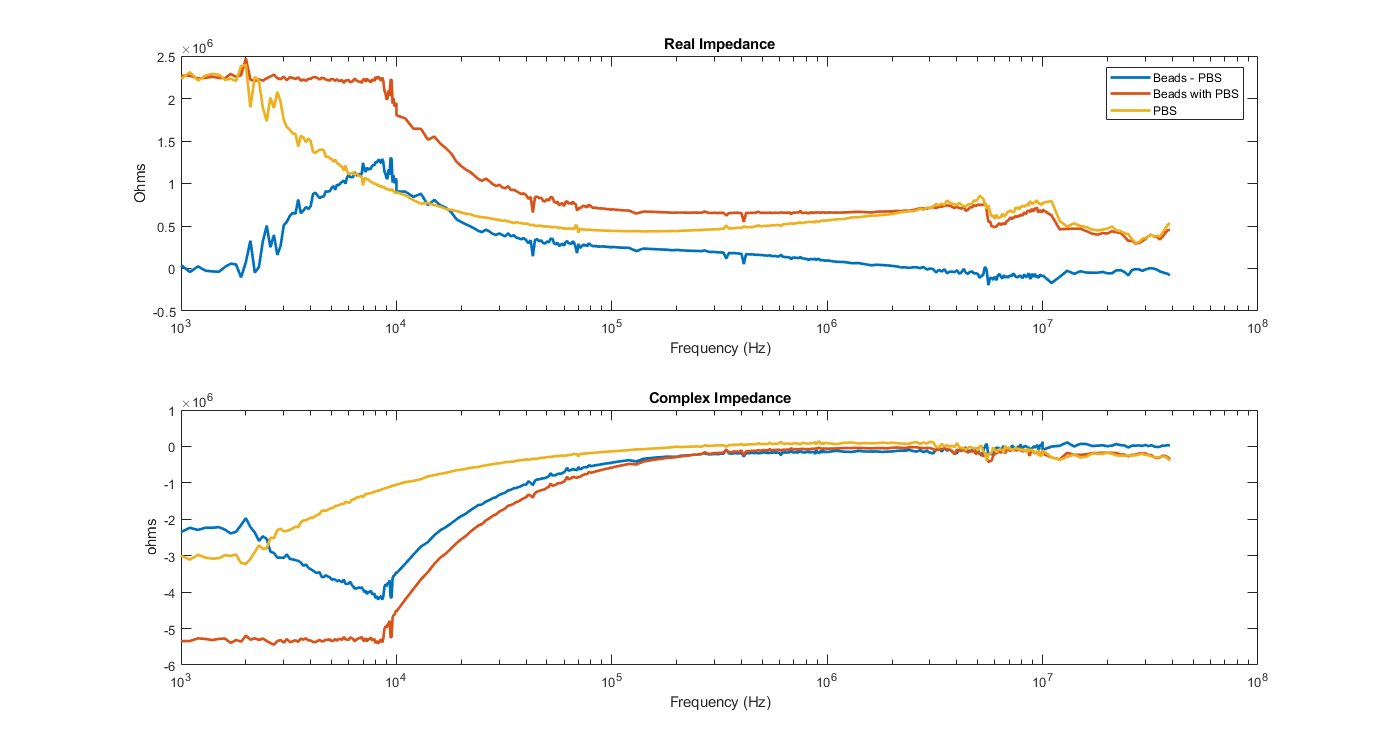
\includegraphics[width=\textwidth]{images/IS_data_clean_real_imag.png}
        \caption{IS results in rectangular form.}
    \end{subfigure}
    \\
    \vspace{0.1 in}
    %\begin{subfigure}[b]{\textwidth}
    %    \centering
    %    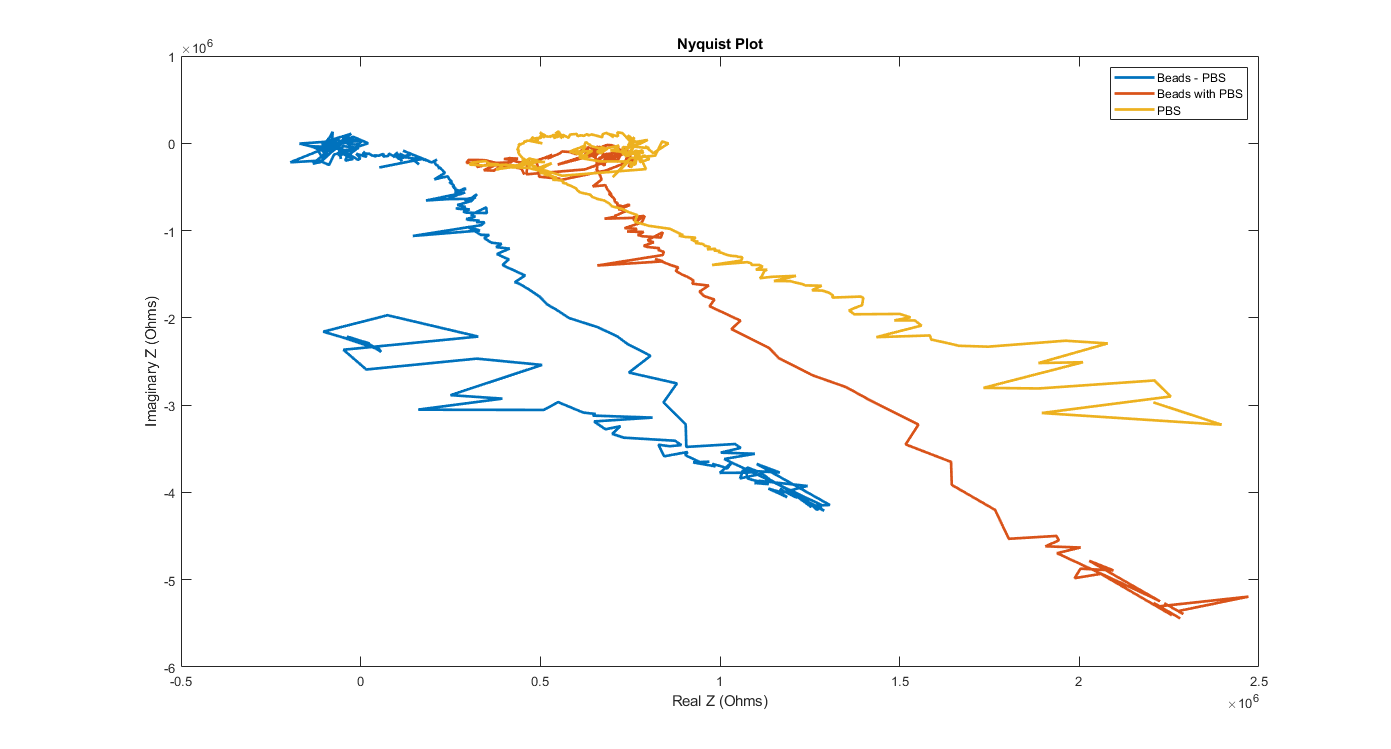
\includegraphics[width=\textwidth]{images/IS_data_clean_nyquist.png}
    %    \caption{Jammed}
    %\end{subfigure}
    \caption[PBS, PBS saturated with micro-beads, and the phasor difference.]{Comparison of impedance spectroscopy results from measurements of phosphate buffered solution, phosphate buffered solution saturated with 7 $\mu$m polystyrene beads, and the phasor difference between the two. The phase data was cleaned and the real and imaginary impedance was re-calculated.}
    \label{fig:IS_data_pbs_pbsBeads_difference}
\end{figure}

\begin{figure}[h]
    \centering
    \begin{subfigure}[b]{\textwidth}
        \centering
        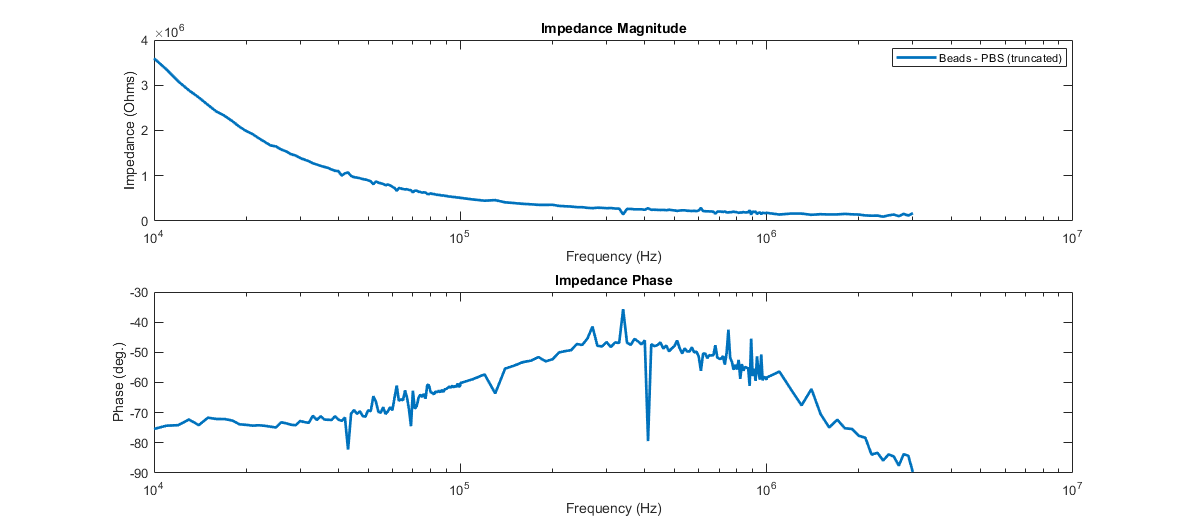
\includegraphics[width=\textwidth]{images/IS_data_beads-PBS_truncated_mag_phase.png}
        \caption{Impedance spectra phasor difference in polar form.}
    \end{subfigure}
    \\
    \vspace{0.1 in}
    \begin{subfigure}[b]{\textwidth}
        \centering
        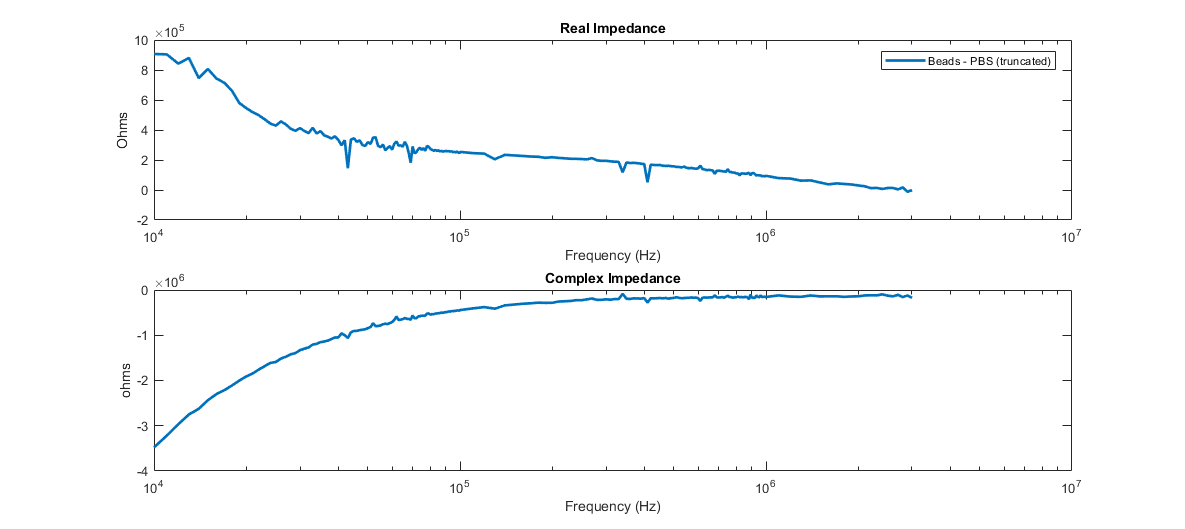
\includegraphics[width=\textwidth]{images/IS_data_beads-PBS_truncated_real_imag.png}
        \caption{Impedance spectra phasor difference in rectangular form.}
    \end{subfigure}
    \\
    %\vspace{0.1 in}
    %\begin{subfigure}[b]{\textwidth}
    %    \centering
    %    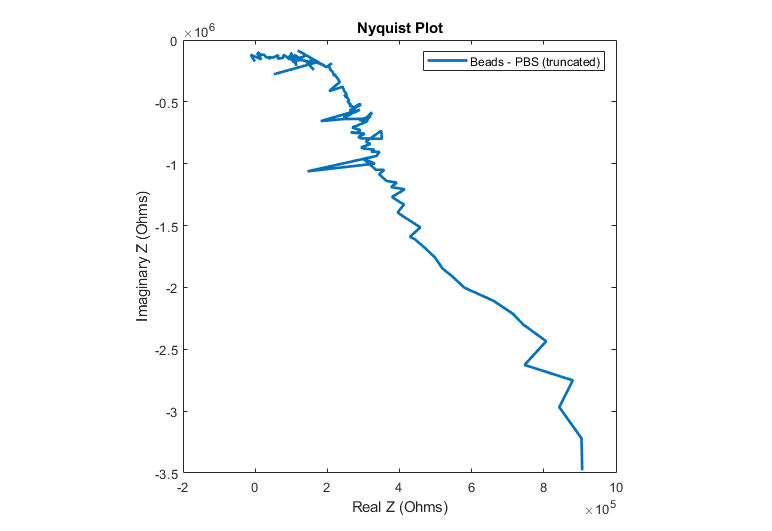
\includegraphics[width=\textwidth]{images/IS_data_beads-PBS_nyquist.png}
    %    \caption{Jammed}
    %\end{subfigure}
    \caption[Truncated phasor difference between PBS, and micro-bead saturated PBS.]{Phasor difference between the PBS solution, and PBS solution saturated with 7$\mu$m microbeads. The data was truncated to the reliable frequency range of $10^4$ to $3x10^6$ hz.}
    \label{fig:IS_data_beads_pbs_DI_comp}
\end{figure}


\FloatBarrier

\section{Modeling}

\subsection{Impedance Spectroscopy Results}

\begin{figure}[h]
    \centering
    \begin{subfigure}[b]{\textwidth}
        \centering
        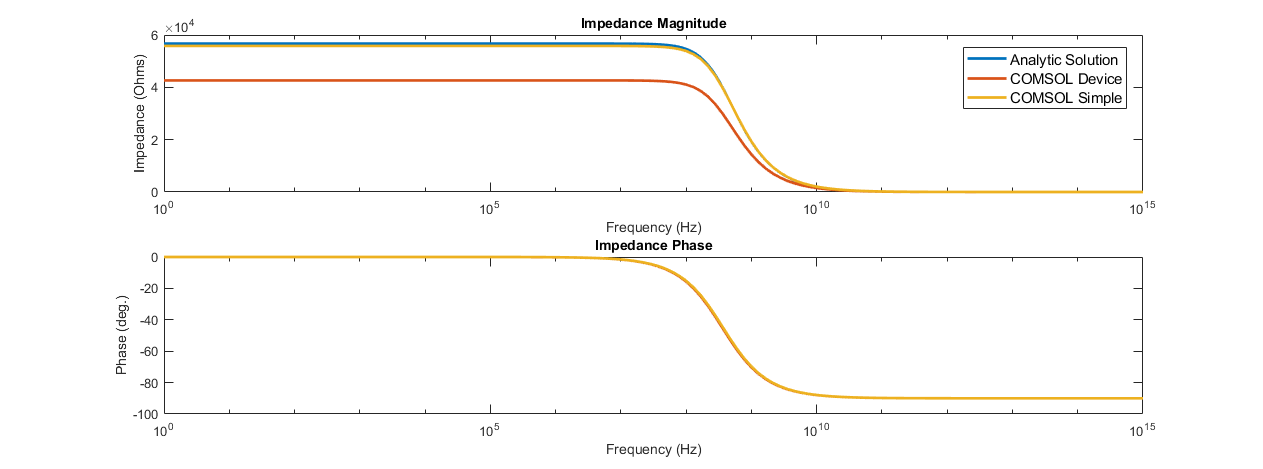
\includegraphics[width=\textwidth]{images/IS_model_medium_mag_phase.png}
        \caption{Impedance spectra in polar form.}
    \end{subfigure}
    \\
    \vspace{0.1 in}
    \begin{subfigure}[b]{\textwidth}
        \centering
        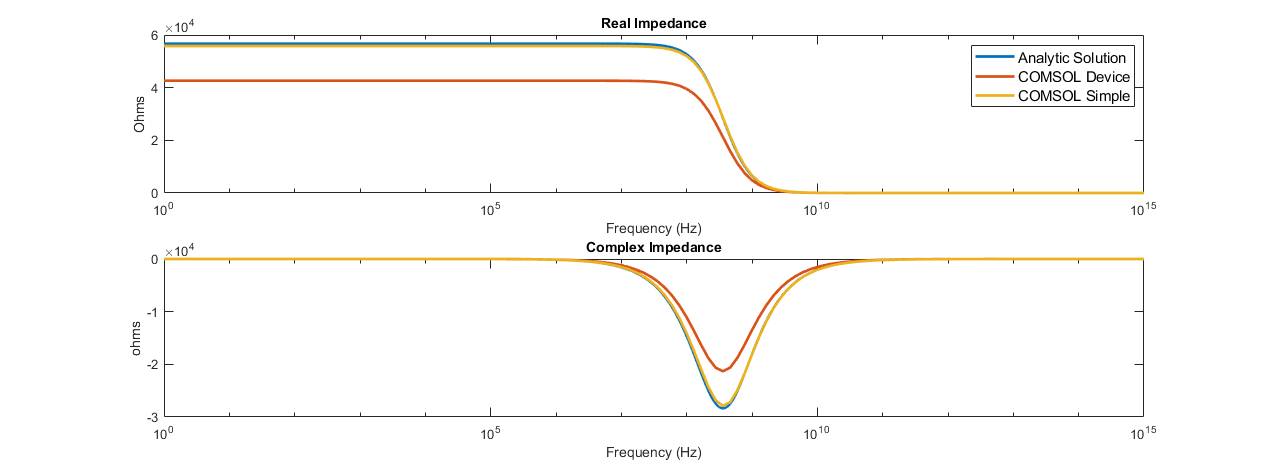
\includegraphics[width=\textwidth]{images/IS_model_medium_real_imag.png}
        \caption{Impedance spectra in rectangular form.}
    \end{subfigure}
    \\
    \vspace{0.1 in}
%    \begin{subfigure}[b]{\textwidth}
 %       \centering
  %      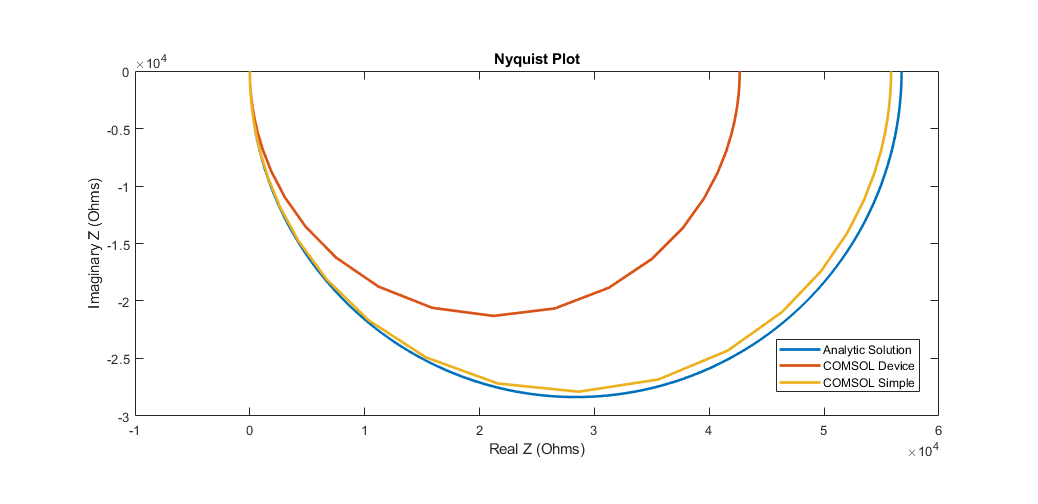
\includegraphics[width=\textwidth]{images/IS_model_medium_nyquist.png}
   %     \caption{Jammed}
    %\end{subfigure}
    \caption[Analyitic and FEA generated medium impedance spectrum]{Medium impedance spectrum generated by the analytic impedance solution, the simple FEA model, and the device FEA model.}
    \label{fig:medium_model_IS_data}
\end{figure}

\begin{figure}[h]
    \centering
    \begin{subfigure}[b]{\textwidth}
        \centering
        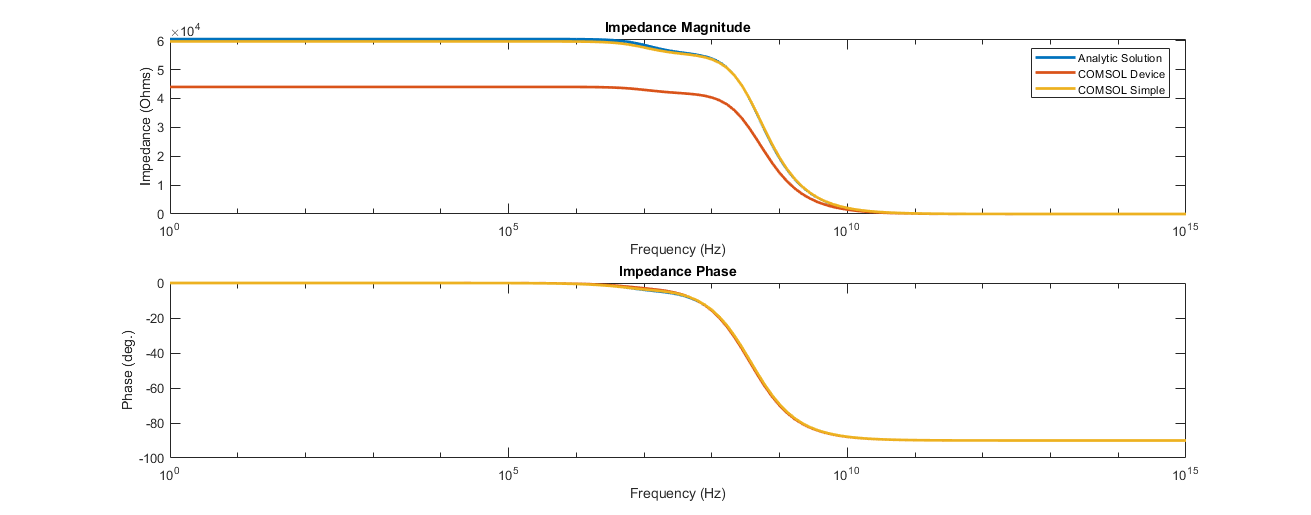
\includegraphics[width=\textwidth]{images/IS_model_mag_phase.png}
        \caption{Impedance spectra in polar form.}
    \end{subfigure}
    \\
    \vspace{0.1 in}
    \begin{subfigure}[b]{\textwidth}
        \centering
        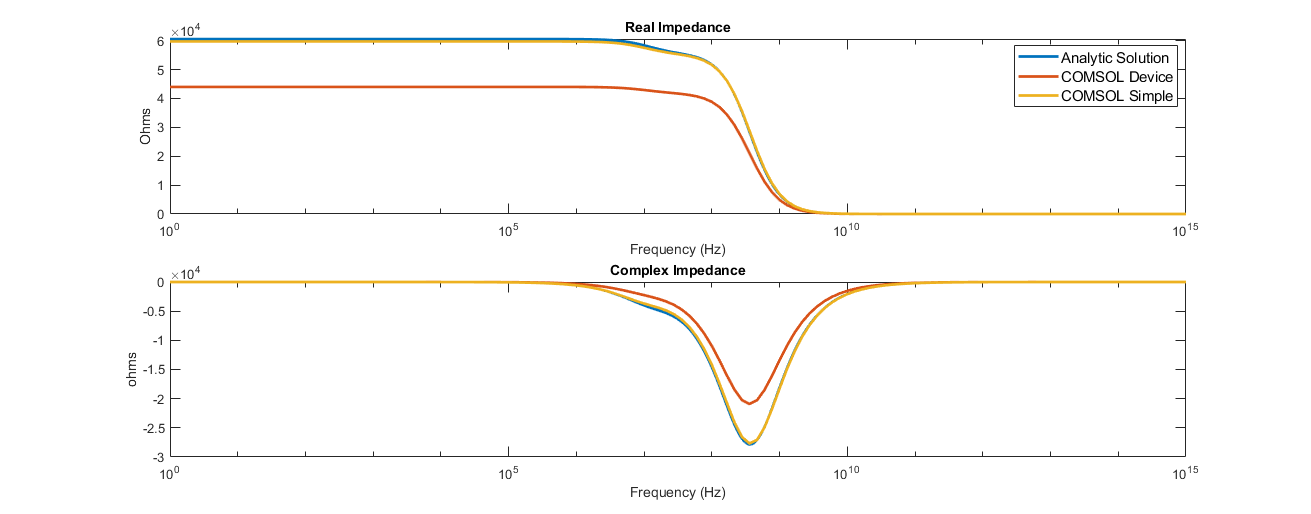
\includegraphics[width=\textwidth]{images/IS_model_real_imag.png}
        \caption{Impedance spectra in rectangular form.}
    \end{subfigure}
    %\\
    %\vspace{0.1 in}
    %\begin{subfigure}[b]{\textwidth}
      %  \centering
     %   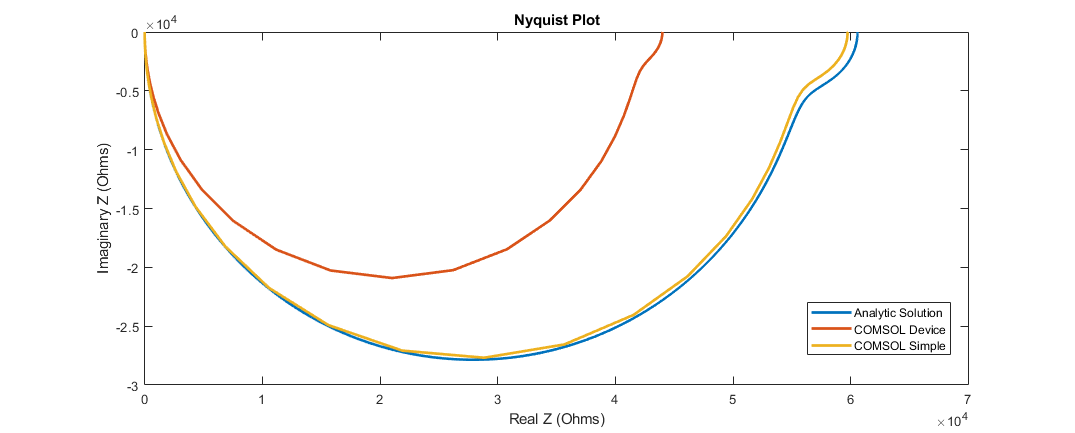
\includegraphics[width=\textwidth]{images/IS_model_nyquist.png}
%        \caption{Jammed}
%    \end{subfigure}
    \caption[Analyitic and FEA generated single cell impedance spectrums]{Single cell impedance spectrum generated by the analytic impedance solution, the simple FEA model, and the device FEA model.}
    \label{fig:single_cell_model_IS_data}
\end{figure}

\begin{figure}[h]
    \centering
    \begin{subfigure}[b]{\textwidth}
        \centering
        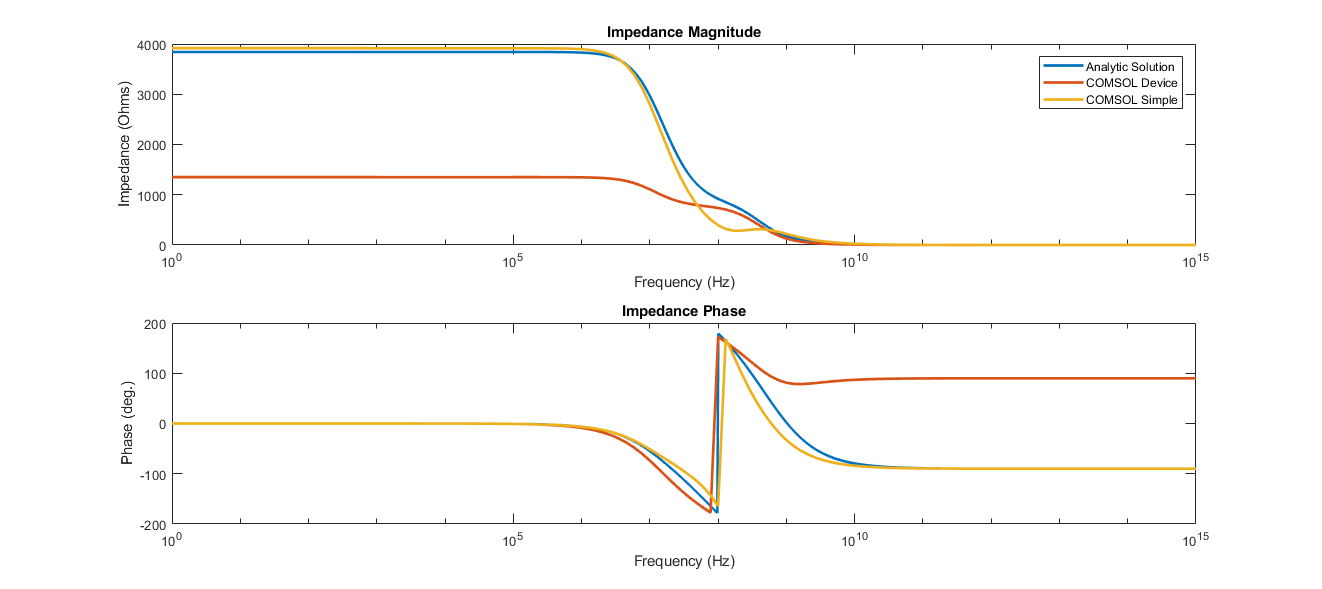
\includegraphics[width=\textwidth]{images/IS_model_difference_mag_phase.png}
        \caption{Impedance spectra in polar form.}
    \end{subfigure}
    \\
    \vspace{0.1 in}
    \begin{subfigure}[b]{\textwidth}
        \centering
        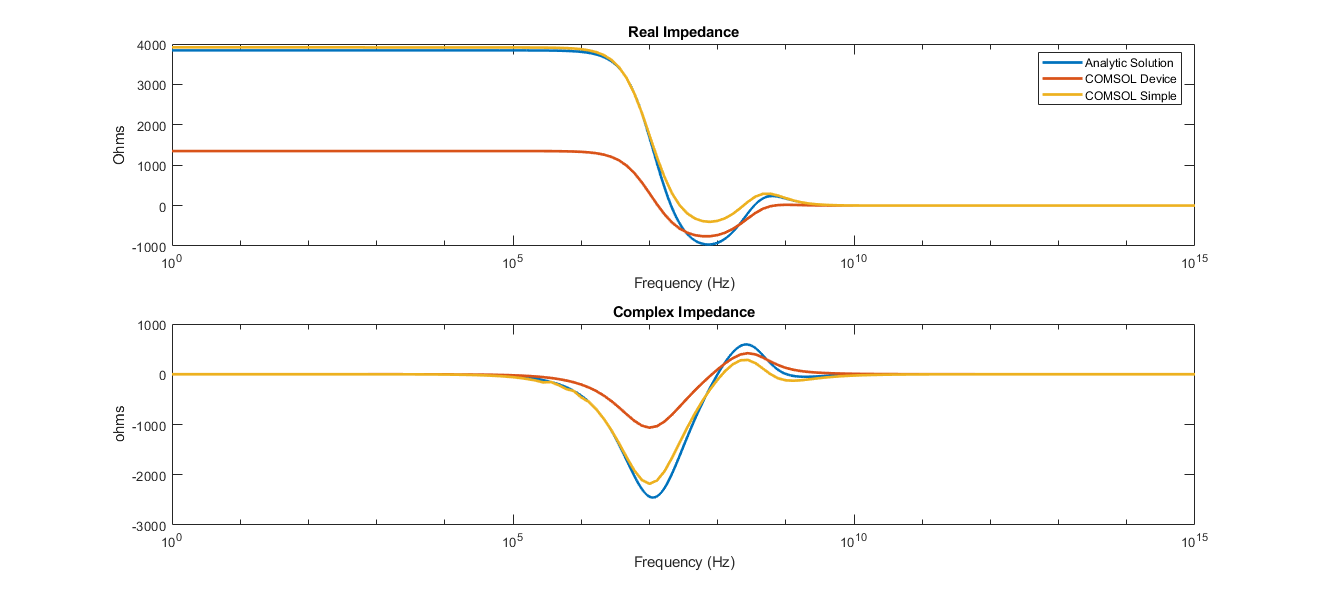
\includegraphics[width=\textwidth]{images/IS_model_difference_real_imag.png}
        \caption{Impedance spectra in rectangular form.}
    \end{subfigure}
%    \\
%    \vspace{0.1 in}
%    \begin{subfigure}[b]{\textwidth}
%        \centering
%        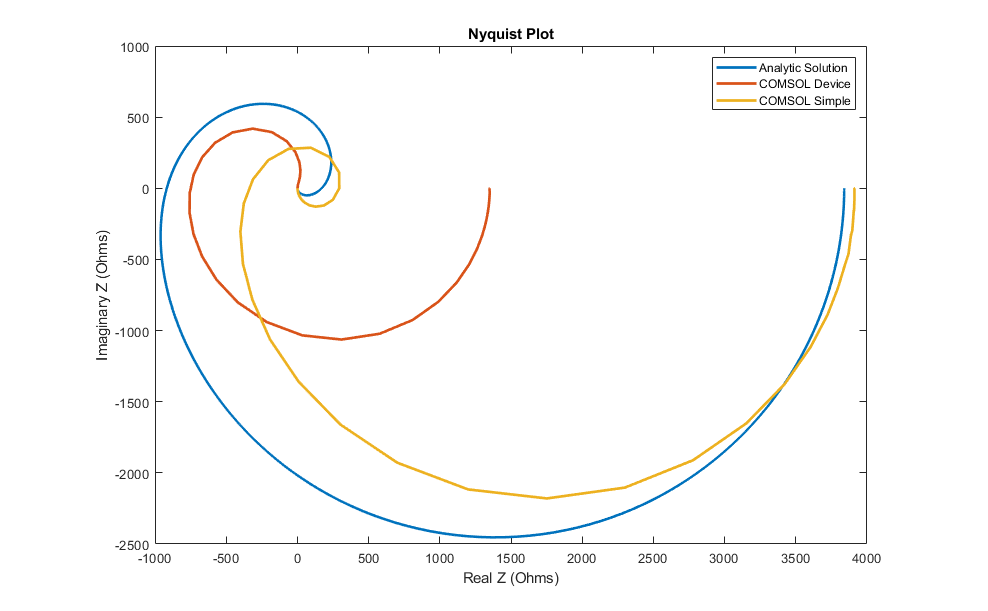
\includegraphics[width=\textwidth]{images/IS_model_difference_nyquist.png}
%        \caption{Jammed}
%    \end{subfigure}
    \caption[Phasor difference between model mixture and medium impedance spectrum.]{Phasor difference between model mixture and medium impedance spectrum generated by the analytic impedance solution, the simple FEA model, and the device FEA model.}
    \label{fig:single_cell_model_IS_data}
\end{figure}

\begin{figure}[h]
    \centering
    \begin{subfigure}[b]{\textwidth}
        \centering
        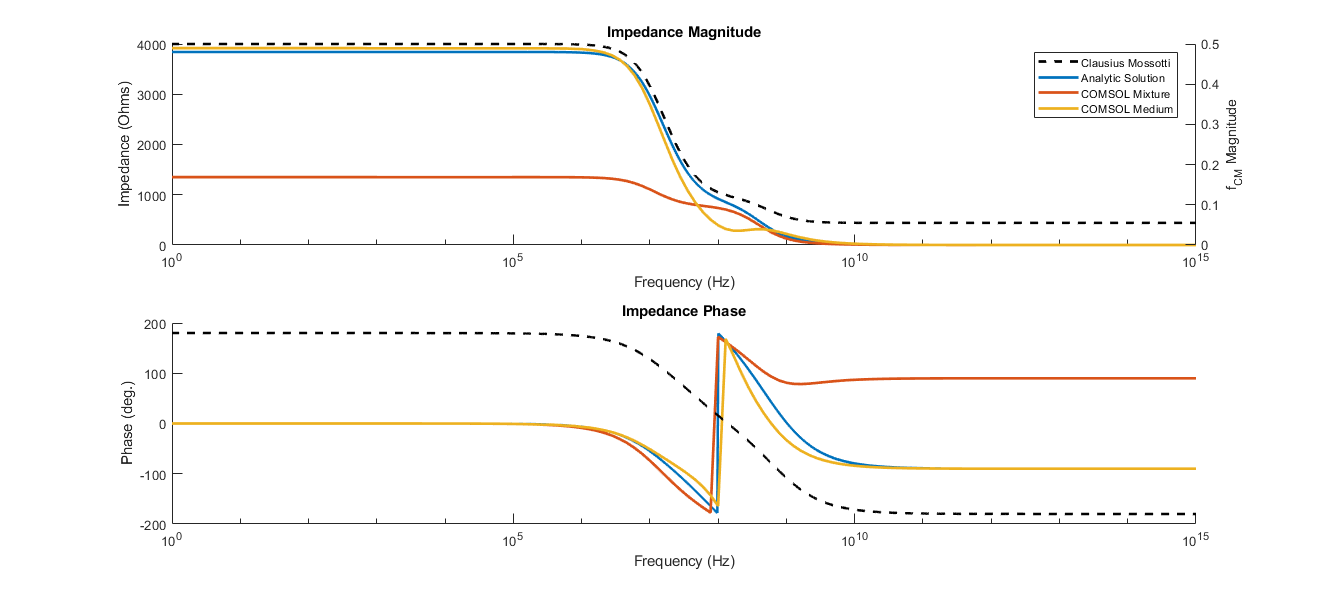
\includegraphics[width=\textwidth]{images/IS_model_difference_mag_phase_CM_overlay.png}
        \caption{Clausius Mossotti factor overlaid on difference impedance in polar form.}
    \end{subfigure}
    \\
    \vspace{0.1 in}
    \begin{subfigure}[b]{\textwidth}
        \centering
        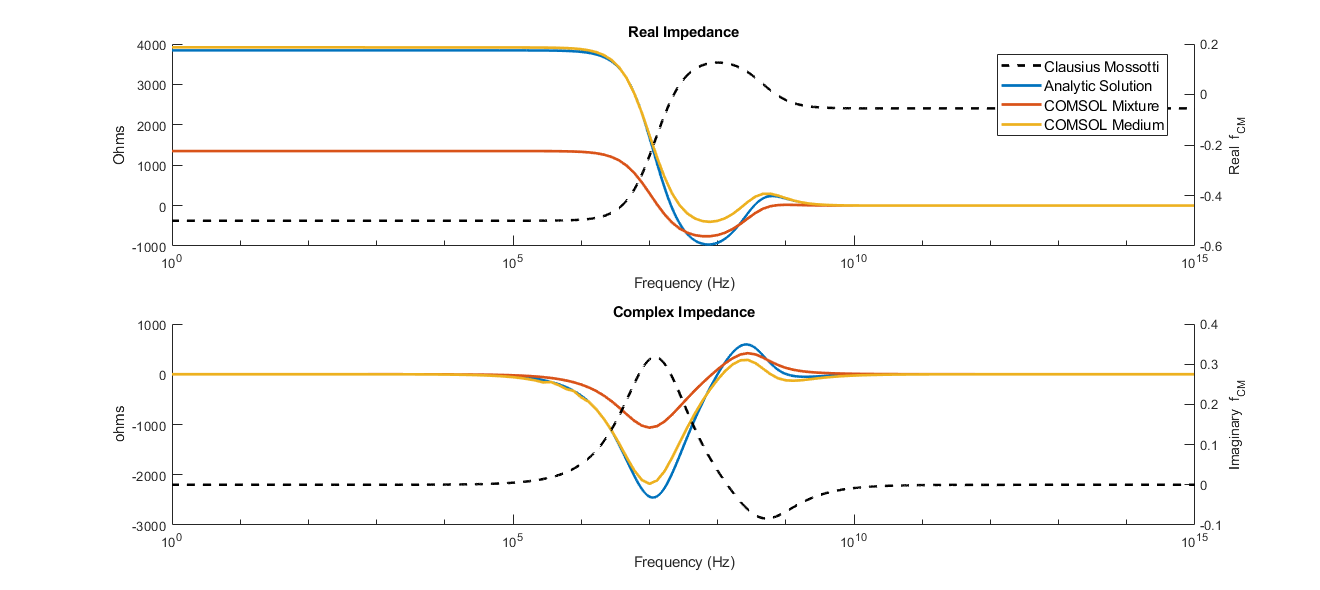
\includegraphics[width=\textwidth]{images/IS_model_real_imag_difference_CM_overlay.png}
        \caption{Clausius Mossotti factor overlaid on difference impedance in rectangular form.}
    \end{subfigure}

    \caption[Clausius Mossotti factor overlaid on IS model data.]{Clausius Mossotti factor overlaid on phasor difference between mixture and medium impedance spectrum model data generated from the analytic solution, the simple FEA model, and the device FEA model. It is clearly depicted how the impedance spectra tracks Clausius Mossotti factor, and illustrates how the impedance responds to cell-medium dielectric dispersions.}
    \label{fig:IS_model_difference_fcm_overlay}
\end{figure}

\begin{figure}[h]
    \centering
    \begin{subfigure}[b]{\textwidth}
        \centering
        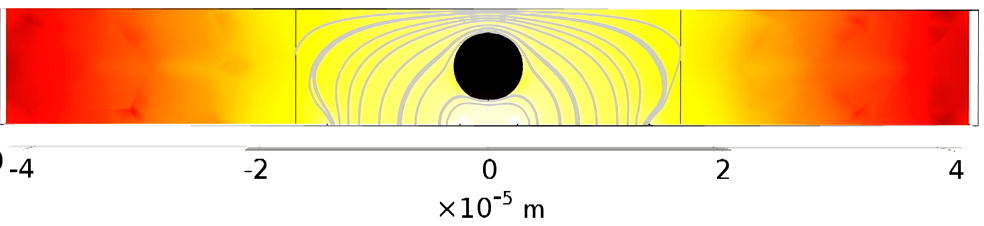
\includegraphics[width=\textwidth]{images/simple_cell_DC.png}
        \caption{The electric field at DC.}
    \end{subfigure}
    \\
    \vspace{0.1 in}
    \begin{subfigure}[b]{\textwidth}
        \centering
        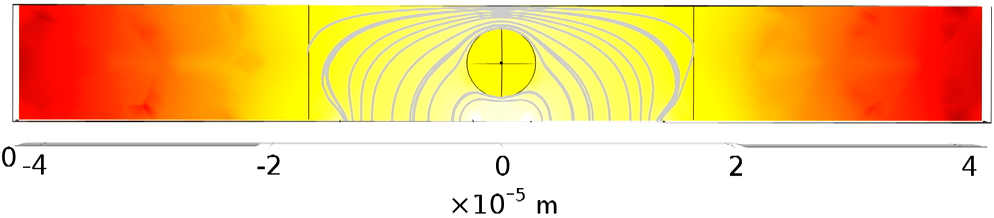
\includegraphics[width=\textwidth]{images/simple_cell_1Mhz.png}
        \caption{The electric field at 1 Mhz. Need to consider where membrane and cytoplasm relaxation occurs}
    \end{subfigure}
    \\
    \vspace{0.1 in}
    \begin{subfigure}[b]{\textwidth}
        \centering
        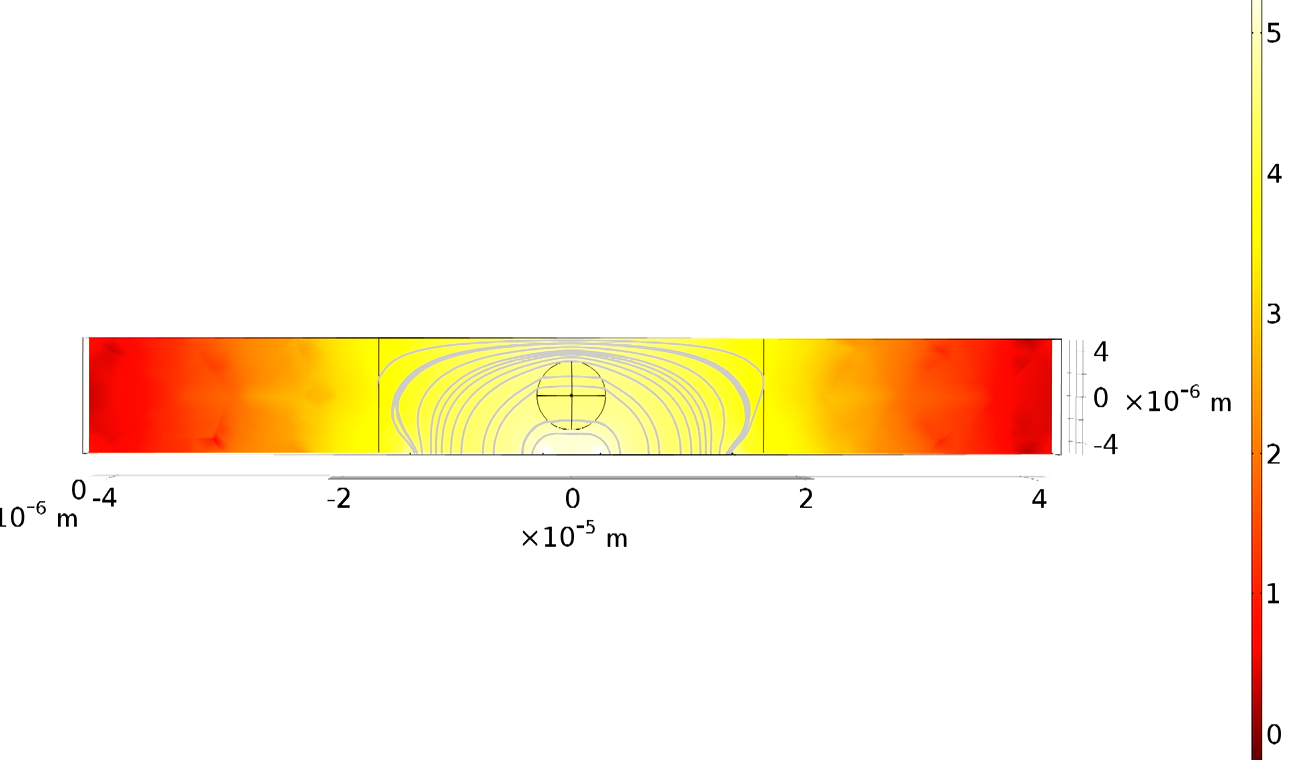
\includegraphics[width=\textwidth]{images/simple_cell_10Mhz.png}
        \caption{The electric field magnitudes and isolines at 10 Mhz. The Maxwell-Wagner relaxation has taken affect as demonstrated by electric field line penetration of the cell.}
    \end{subfigure}
        \\
    \vspace{0.1 in}
    \begin{subfigure}[b]{\textwidth}
        \centering
        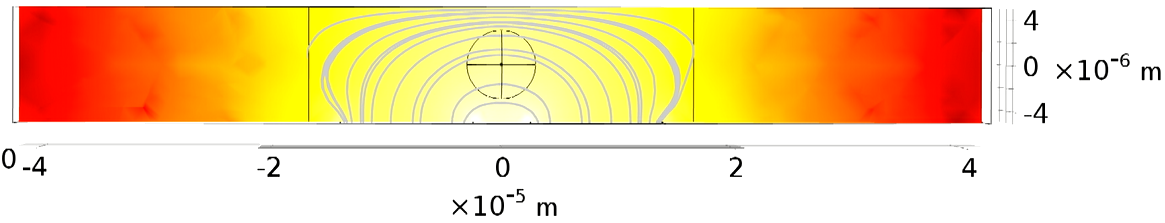
\includegraphics[width=\textwidth]{images/simple_cell_1Ghz.png}
        \caption{The electric field at 1 GHz.}
    \end{subfigure}
        \\
    \vspace{0.1 in}
    \begin{subfigure}[b]{\textwidth}
        \centering
        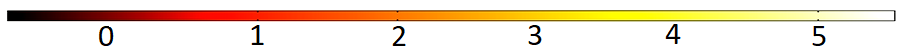
\includegraphics[width=\textwidth]{images/simpleCellColorMapAxis.png}
        \caption{The color map axis describing the magnitude of the electric field for the preceding sub-figures as log$_{10}(V/m)$.}
    \end{subfigure}
    \caption[FEA simple model electric field surface plot.]{FEA simple model plots of the electric field at frequencies of interest. The logarithm of the electric field magnitude is depicted through the color mapping outlined by the color axis in sub-figure (e), and the electric field lines are illustrated with white curves in the region of the electrodes and cell.}
    \label{fig:single_cell_model_EZ_plots}
\end{figure}

\begin{figure}[h]
    \centering
    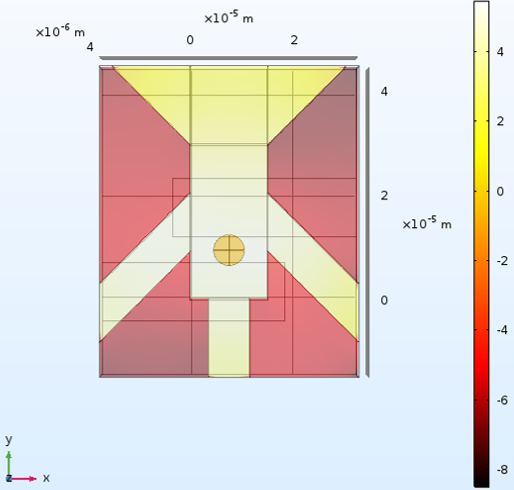
\includegraphics[width=0.7\textwidth]{images/deviceCellCurrent1Hz.png}
    \caption[Current density plot of the FEA device model.]{Current density plot of the FEA device model at DC. The color mapping depicts the logarithm of the current density magnitude.}
    \label{fig:device_current_denisty plot}
\end{figure}

Discuss the calculated device inefficiency.

\FloatBarrier

\subsection{optimization}



\begin{figure}[h]
    \centering
    \begin{subfigure}[t]{0.49\textwidth}
        \centering
        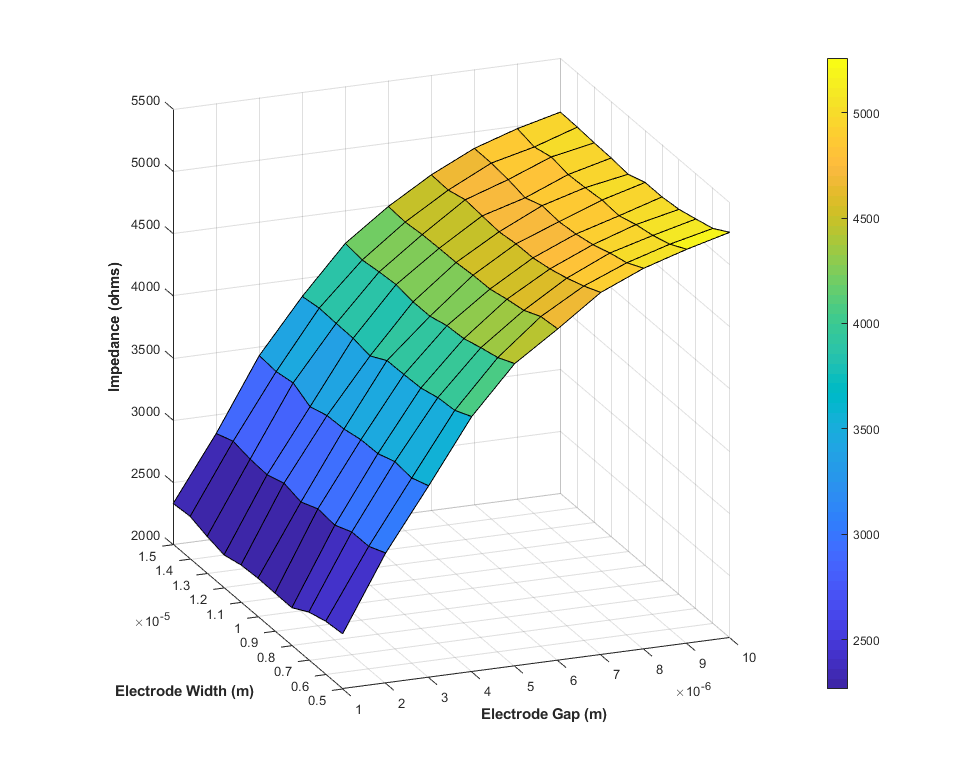
\includegraphics[width=\textwidth]{images/comsol_simple_difference.png}
        \caption{Impedance difference curve.}
    \end{subfigure}
    \hfill
    \begin{subfigure}[t]{0.49\textwidth}
        \centering
        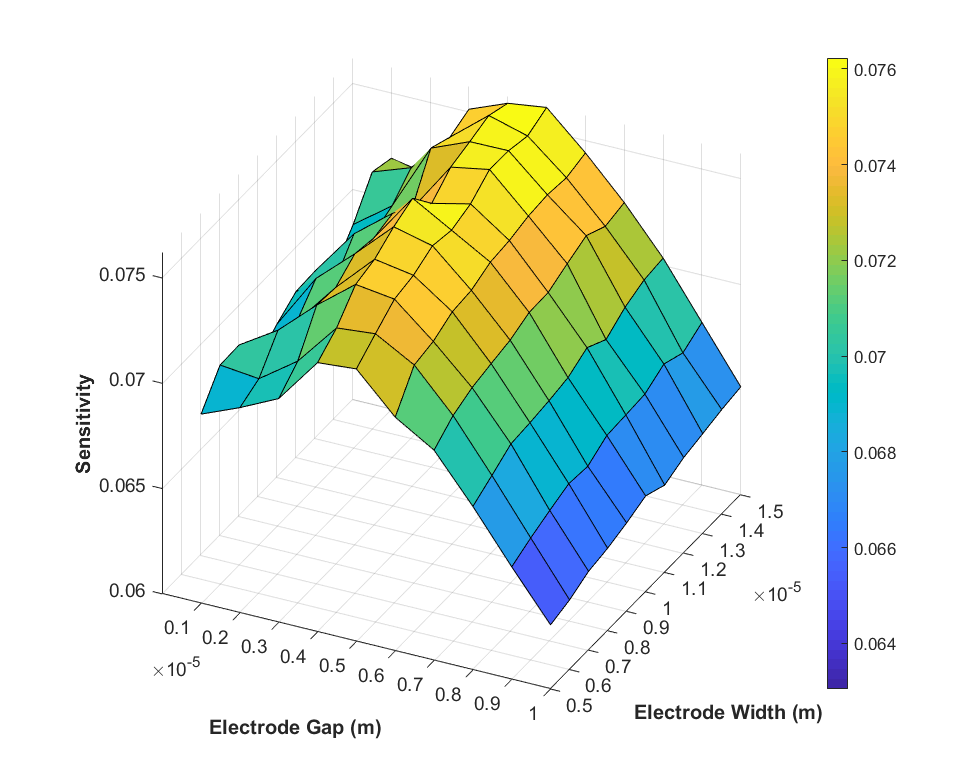
\includegraphics[width=\textwidth]{images/comsol_simple_sensitivity_surface.png}
        \caption{Impedance sensitivity curve.}
    \end{subfigure}
    \\
    \vspace{0.1 in}
    \begin{subfigure}[t]{0.49\textwidth}
        \centering
        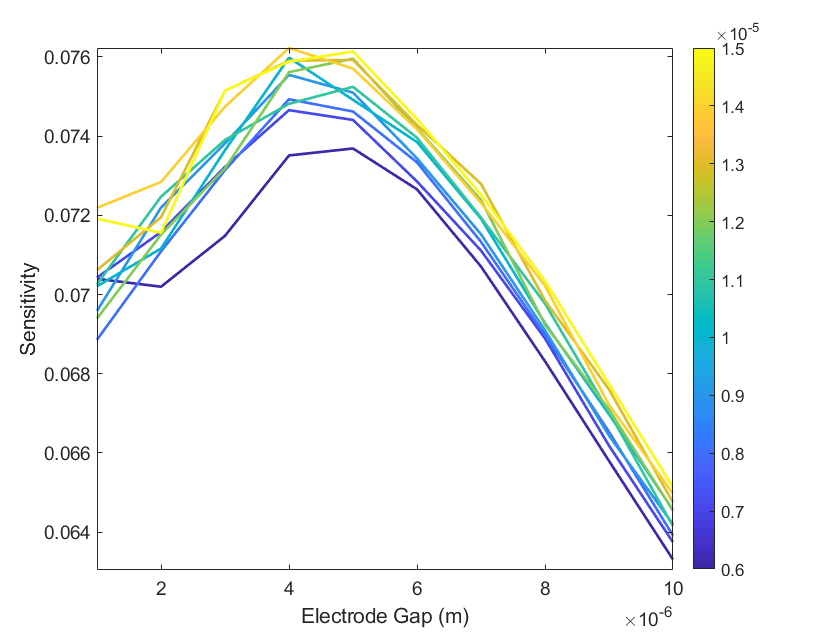
\includegraphics[width=\textwidth]{images/comsol_simple_gapXsensitivity.png}
        
        
        
        \caption{Sensitivity vs. gap.}
    \end{subfigure}
    \hfill
    \begin{subfigure}[t]{0.49\textwidth}
        \centering
        \includegraphics[width=\textwidth]{images/comsol_simple_widthXsensitivity.png}
        \caption{Sensitivity vs. width.}
    \end{subfigure}
    \caption[Simple FEA model sensitivity]{Parametric study on device sensitivity using the Simple FEA model. The study varied the electrode width and gap from 5 $\mu$m to 15 $\mu$m and 1 $\mu$m to 10 $\mu$m respectively. The Simple FEA model held a channel height of 10 $\mu$m and a cell centered between the two electrodes with a center height of 5 $\mu$m. The sensitivity was calculated with equation \ref{eqn:Sun_sensitivity}. See section \ref{sec: FEA} for additional details on the Simple FEA model.} 
    \label{fig:simple_sensitivity}
\end{figure}

\par (better for the discussion?) The impedance difference plot was included to show that although there is a peak for the maximum sensitivity, the impedance difference plateaus to a maximum as the electrode gap increases. The impedance difference and Sun's sensitivity tell us two different things: where the sensitivity is a ratio of the difference impedance to the medium impedance, the simple difference impedance gives us insight into the amount of non-relative amount of signal is from the cell. Depending on designer's goal, it may make sense to maximize your signal instead of your sensitivity, or to find a mixture of the two. 

\par It should be noted that the sensitivity curve for the FEA models is significantly "noisier" than the difference curves. This is likely due to "mesh noise". COMSOL generates a new mesh for each simulation in the parametric study. What is referred to as "mesh noise" is the accumulation of effects on results caused by differences in meshes. The appearance of "mesh noise" is a clear signal that the meshing scheme needs to revisited, as the purpose of mesh refinement is to remove the effect of meshes from the model. In this case, the mesh refinement was limited by system running COMSOL, but is definitely an area of future improvement. The sensitivity curves appear noisier due to the magnification of mesh noise from the extra operation on the results.

\begin{figure}[h]
    \centering
    \begin{subfigure}[b]{0.49\textwidth}
        \centering
        \includegraphics[width=\textwidth]{images/comsol_device_surface_difference.png}
        \caption{Difference}
    \end{subfigure}
    \hfill
    \begin{subfigure}[b]{0.49\textwidth}
        \centering
        \includegraphics[width=\textwidth]{images/comsol_device_surface_sensitivity.png}
        \caption{Sensitivity}
    \end{subfigure}
    \\
    \vspace{0.1 in}
    \begin{subfigure}[b]{0.49\textwidth}
        \centering
        \includegraphics[width=\textwidth]{images/comsol_device_gapXsensitivity.png}
        \caption{gap}
    \end{subfigure}
    \hfill
    \begin{subfigure}[b]{0.49\textwidth}
        \centering
        \includegraphics[width=\textwidth]{images/comsol_device_widthXsensitivity.png}
        \caption{width}
    \end{subfigure}
    \caption[Device sensitivity]{Device sensitivity}
    \label{fig:device_sensitivity}
\end{figure}

\begin{figure}[h]
    \centering
    \begin{subfigure}[b]{0.49\textwidth}
        \centering
        \includegraphics[width=\textwidth]{images/comsol_device_gapXsensitivity_aveError.png}
        \caption{Gap}
    \end{subfigure}
    \hfill
    \begin{subfigure}[b]{0.49\textwidth}
        \centering
        \includegraphics[width=\textwidth]{images/comsol_device_widthXsensitivity_aveError.png}
        \caption{Width}
    \end{subfigure}
    \caption[Device sensitivity average]{Device sensitivity average}
    \label{fig:device_sensitivity_average}
\end{figure}

\begin{figure}[h]
    \centering
    \begin{subfigure}[b]{0.49\textwidth}
        \centering
        \includegraphics[width=\textwidth]{images/analytic_difference.png}
        \caption{Difference}
    \end{subfigure}
    \hfill
    \begin{subfigure}[b]{0.49\textwidth}
        \centering
        \includegraphics[width=\textwidth]{images/analytic_sun_surface.png}
        \caption{Sensitivity}
    \end{subfigure}
    \\
    \vspace{0.1 in}
    \begin{subfigure}[b]{0.49\textwidth}
        \centering
        \includegraphics[width=\textwidth]{images/analytic_sun_gapXsensitivity.png}
        \caption{gap}
    \end{subfigure}
    \hfill
    \begin{subfigure}[b]{0.49\textwidth}
        \centering
        \includegraphics[width=\textwidth]{images/analytic_sun_widthXsensitivity.png}
        \caption{width}
    \end{subfigure}
    \caption[Analytic Sensitivity]{Analytic Sensitivity}
    \label{fig:analytic_sensitivity}
\end{figure}

\begin{figure}[h]
    \centering
    \begin{subfigure}[b]{0.49\textwidth}
        \centering
        \includegraphics[width=\textwidth]{images/analytic_sun_difference_expanded.png}
        \caption{Difference}
    \end{subfigure}
    \hfill
    \begin{subfigure}[b]{0.49\textwidth}
        \centering
        \includegraphics[width=\textwidth]{images/analytic_sun_surface_expanded.png}
        \caption{Sensitivity}
    \end{subfigure}
    \\
    \vspace{0.1 in}
    \begin{subfigure}[b]{0.49\textwidth}
        \centering
        \includegraphics[width=\textwidth]{images/analytic_sun_gapXsensitivity_extended.png}
        \caption{gap}
    \end{subfigure}
    \hfill
    \begin{subfigure}[b]{0.49\textwidth}
        \centering
        \includegraphics[width=\textwidth]{images/analytic_sun_widthXsensitivity_extended.png}
        \caption{width}
    \end{subfigure}
    \caption[Analytic Sensitivity]{Analytic Sensitivity}
    \label{fig:analytic_sensitivity}
\end{figure}

\begin{figure}[h]
    \centering
    \begin{subfigure}[b]{0.49\textwidth}
        \centering
        \includegraphics[width=\textwidth]{images/analytic_power_surface.png}
        \caption{Power Surface}
    \end{subfigure}
    \hfill
    \begin{subfigure}[b]{0.49\textwidth}
        \centering
        \includegraphics[width=\textwidth]{images/analytic_gapXpower.png}
        \caption{GapXpower by width}
    \end{subfigure}
    \\
    \vspace{0.1 in}
    \begin{subfigure}[b]{0.49\textwidth}
        \centering
        \includegraphics[width=\textwidth]{images/analytic_widthXpowerByHeight.png}
        \caption{width x power by height}
    \end{subfigure}
    \hfill
    \begin{subfigure}[b]{0.49\textwidth}
        \centering
        \includegraphics[width=\textwidth]{images/analytic_heightXpowerByGap.png}
        \caption{height x power by gap}
    \end{subfigure}
    \caption[power comp]{power comp}
    \label{fig:analytic_sensitivity}
\end{figure}


\begin{figure}[h]
    \centering
    \begin{subfigure}[b]{0.49\textwidth}
        \centering
        \includegraphics[width=\textwidth]{images/analytic_vertical_power.png}
        \caption{Power Surface}
    \end{subfigure}
    \hfill
    \begin{subfigure}[b]{0.49\textwidth}
        \centering
        \includegraphics[width=\textwidth]{images/analytic_horizontal_power.png}
        \caption{GapXpower by width}
    \end{subfigure}
    \\
    \vspace{0.1 in}
    \begin{subfigure}[b]{0.49\textwidth}
        \centering
        \includegraphics[width=\textwidth]{images/analytic_vertical_power_width20.png}
        \caption{width x power by height}
    \end{subfigure}
    \hfill
    \begin{subfigure}[b]{0.49\textwidth}
        \centering
        \includegraphics[width=\textwidth]{images/analytic_horizontal_power_20width.png}
        \caption{height x power by gap}
    \end{subfigure}
    \caption[power comp]{power comp}
    \label{fig:analytic_sensitivity}
\end{figure}

\FloatBarrier

\section{IS DAQ Validation and Measurement Analysis}

\par To validate and investigate the impedance spectroscopy DAQ system, the test circuit in figure \ref{fig:IS_DAQ_test_circuit} was physically implemented and tested, and simulated in SPICE with and without oscilloscopes. As illustrated in the bode plot of figure \ref{fig:test_circuit_bode} and the impedance spectra of \ref{fig:test_circuit_impedance_spectra}, the measured data and the SPICE model with scopes data largely matched. However, there were large deviations from the ideal SPICE model without any of the limitations of a DAQ system. This demonstrates how the application of passive oscilloscopes with the I-V method can cause large errors that grow with higher frequencies. Rerffering to figure \ref{fig:IS_DAQ_test_circuit}, oscilloscope 1 attached to V1 has very little effects on the I-V results, however, part of the I-V method is the assumption that all current flowing through the DUT is also flowing through the external resistor $R_{EXT}$. With the connection of oscilloscope 2 to node V2, this is no longer true, and as the applied frequency increases, non-negligible current leaks through the oscilloscope's capacitance. The percent error of the in figure \ref{fig:test_circuit_bode}. Although it is true that the error 

\par Figure \ref{fig:test_circ_measurement_error} also demonstrates, that although the modelled limitations of the passive probes used accounts for a significant amount of the IS DAQ error, there are unaccounted effect. At low frequencies, the recorded data reports an error on the magnitude of 10\% whereas the oscilloscope simulation reported an error on the magnitude of 3\%. In addition, starting at frequencies of 6 MHz, the measured data depicts further deviations. The low frequency errors may be attributed to a myriad of reason including the parasitic capacitance of the breadboard, and deviations in the actual versus reported values of the oscilloscope's, external resistor's, and test capacitor's capacitance and resistance. The high frequency deviations may be due to parasitic inductance in the system that is unaccounted for in the SPICE models.

\par With this empirical confirmation, a corrective term can be derived to adjust the measured impedance spectra to a corrected impedance spectra. Revisiting the impedance solution for I-V method we have 
\begin{equation}
    Z_{DUT} = \frac{V_1 - V_2}{I}.
\end{equation}

\par In ideal scenarios, we would assume all current flows through the external resistor and then $I = V_2 / R_{EXT}$. However, we know that is not true: the non-ideal properties allows current to flow through our attached oscilloscopes and this current must be accounted for. 
\begin{equation}
    Z_{DUT} = \bigg(\frac{V_1 - V_2}{V_2}\bigg)Z_{EXT},
    \label{eqn:corrected_IV}
\end{equation}
\noindent where
\begin{equation}
    Z_{EXT} = \bigg(\frac{1}{Z_{scope}}+\frac{1}{R_{EXT}}\bigg)^{-1}.
    \label{eqn:corrected_Rext}
\end{equation}

\par Future impedance spectra can be calculated with equations \ref{eqn:corrected_IV} and \ref{eqn:corrected_Rext}, or non-corrected I-V impedance spectra can be corrected as follows:

\begin{equation}
    Z_{DUT} = Z_{NC}\bigg(\frac{Z_{EXT}}{R_{EXT}}\bigg),
\end{equation}

\noindent Where $Z_{NC}$ is the non-corrected I-V impedance spectra.



\begin{figure}[h]
    \centering
    \includegraphics[width=0.9\textwidth]{images/spice-measured-comp.png}
    \caption{Bode plot of the ratio of the voltage out of the DUT to the voltage in.}
    \label{fig:test_circuit_bode}
\end{figure}



\begin{figure}[H]
\centering
    \begin{subfigure}[b]{\textwidth}
        \centering
        \includegraphics[width=0.9\textwidth]{images/awesome_view.jpg}
        \caption{Ideal test circuit}
    \end{subfigure}
    \\
    \vspace{0.1 in}
    \begin{subfigure}[b]{\textwidth}
        \centering
        \includegraphics[width=0.9\textwidth]{images/awesome_view.jpg}
        \caption{Implemented test circuit}
    \end{subfigure}
    \caption{Circuit measured and modeled. Need to include parameter values. Consider moving to the models section.}
    \label{fig:IS_DAQ_test_circuit}
\end{figure}

\begin{figure}[H]
    \centering
    \begin{subfigure}[b]{\textwidth}
        \centering
        \includegraphics[width=\textwidth]{images/spice-measured-comp_mag-phase.png}
        \caption{Impedance spectra in polar form.}
    \end{subfigure}
    \\
    \vspace{0.1 in}
    \begin{subfigure}[b]{\textwidth}
        \centering
        \includegraphics[width=0.9\textwidth]{images/spice-measured-comp.png}
        \caption{Bode plot of the ratio of the voltage out of the DUT to the voltage in.}
    \end{subfigure}
    \caption[Comparison of measured and simulated response of test circuit.]{A comparison of the measured data, ideal simulation, and simulation with non-ideal scopes. The simulations implemented spice to calculate the test capacitor with I-V method. The measured and modeled test circuit is described in figure \ref{}}
    \label{fig:test_circuit_impedance_spectra}
\end{figure}

\par NOTE: Should go back and look at assumption for EDL values for micro electrodes and calculate what the equivalent capacitor. Compare to the DUT capacitor used. Answer: Using the experimentally determined EDL capacitance for titanium electrodes of 6$\mu$F/cm$^2$, as determined by Gongadze \cite{_gongadze.pdf_????}, and assuming that each electrode has fluid contact area of 11.5$\mu$m by 15$\mu$m, eachn electrode would have a capacitance of 10.35 pF, and system EDL capacitance of 5.175 pF. Using a capacitor of 10 pF is well within the margin of error and should model device response. 

\par NOTE: should add IS data to an circuit overlay. May be similar curve and confirm our assumption.

\par Furthermore, our EDL capacitance assumption is further validated by the overlay of the buffer empirical data.

\par NOTE: Consider error caused by oscilloscopes and compensate real data. In addition, attempt to subtract theoretical capacitance from data.

\par NOTE: Consider adding rectangular impedance data. Illustrates how the oscilliscopes create a phantom resistor that 

\par NOTE: Should validate circuit model is correct by running in spice.

\begin{figure}[H]
    \centering
    \includegraphics[width=\textwidth]{images/measurementError.png}
    \caption{The percent error of the recorded data and the spice model with scopes with respect to the ideal spice model. (Reconsider inclusion)}
    \label{fig:test_circ_measurement_error}
\end{figure}